人类的视觉系统是世界的奇迹之一. 考虑下面这串手写数字：

\begin{center}
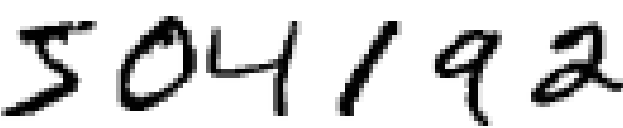
\includegraphics[width=0.267\textwidth]{images/digits.png}
\end{center}

\noindent 大多数人毫不费力地将这些数字识别为 504192. 这种轻松是具有欺骗性的. 在我们大脑的每个半球中，人类都有一个初级视觉皮层，也称为 V1，包含 1.4 亿个神经元\label{term:7}，它们之间有数百亿个连接. 然而人类的视觉不仅仅涉及 V1，还涉及一整套视觉皮层——V2、V3、V4 和 V5——进行着越来越复杂的图像处理. 我们头脑中携带的是一台超级计算机，经过数亿年的进化调校，极其擅长理解视觉世界. 识别手写数字并不容易. 相反，我们人类极其、惊人地擅长理解眼睛所展示给我们的东西. 但几乎所有的工作都是无意识完成的. 因此我们通常不会意识到我们的视觉系统所解决的问题有多么困难.

如果你尝试编写一个计算机程序来识别上面那样的数字，视觉模式识别的困难就会变得显而易见. 当我们自己来做时看似容易的事情，突然变得极其困难. 关于我们如何识别形状的简单直觉——``一个 9 在顶部有一个环，在右下角有一个竖笔画''——结果发现并不那么容易用算法表达. 当你试图使这样的规则精确时，你很快就会迷失在例外、注意事项和特殊情况的泥沼中. 这似乎毫无希望.

神经网络以不同的方式处理这个问题. 其想法是取大量手写数字，称为训练样本\label{term:8}，

\begin{center}
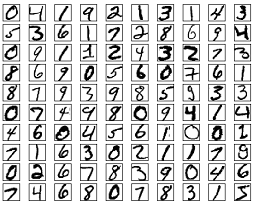
\includegraphics[width=0.733\textwidth]{images/mnist_100_digits.png}
\end{center}

\noindent 然后开发一个能够从这些训练样本中学习的系统. 换句话说，神经网络使用这些样本来自动推断识别手写数字的规则. 此外，通过增加训练样本的数量，网络可以学到更多关于手写的知识，从而提高其准确性. 所以虽然我上面只展示了 100 个训练数字，但也许我们可以通过使用数千甚至数百万或数十亿个训练样本来构建一个更好的手写识别器.

在本章中，我们将编写一个实现神经网络的计算机程序，该网络学习识别手写数字. 这个程序只有 74 行，并且不使用任何特殊的神经网络库. 但这个简短的程序可以在没有人工干预的情况下以超过 96\% 的准确率识别数字. 此外，在后面的章节中，我们将发展一些想法，可以将准确率提高到超过 99\%. 事实上，最好的商业神经网络现在如此之好，以至于银行用它们来处理支票，邮局用它们来识别地址.

我们专注于手写识别，因为它是学习神经网络的一个极好的原型问题. 作为一个原型，它恰好处于一个最佳位置：它具有挑战性——识别手写数字绝非易事——但它又没有难到需要极其复杂的解决方案或巨大的计算能力. 此外，它是发展更先进技术（如深度学习）的好方法. 因此，在整本书中我们将反复回到手写识别的问题上. 在本书后面，我们将讨论这些想法如何应用于计算机视觉中的其他问题，以及语音、自然语言处理和其他领域.

当然，如果本章的目的仅仅是编写一个识别手写数字的计算机程序，那么本章会短得多！但在过程中我们将发展许多关于神经网络的关键思想，包括两种重要类型的人工神经元\label{term:11}（感知机和 S 型神经元），以及神经网络的标准学习算法\label{term:12}，称为随机梯度\label{term:13}下降\label{term:10}\label{term:9}. 在整个过程中，我专注于解释\emph{为什么}事情要这样做，以及建立你的神经网络直觉. 这需要比仅仅展示基本机制更长的讨论，但为了你将获得的更深入理解，这是值得的. 其中的收获之一是，到本章结束时，我们将能够理解什么是深度学习，以及它为什么重要.
\sectionTitle{感知机}{感知机}

什么是神经网络？为了入门，我将解释一种称为\emph{感知机}（perceptron）\label{term:3}的人工神经元. 感知机由科学家 Frank Rosenblatt 在 20 世纪 50 年代和 60 年代开发，灵感来自 Warren McCulloch 和 Walter Pitts 的早期工作. 如今，使用其他人工神经元模型更为常见——在本书中，以及在许多现代神经网络工作中，使用的主要神经元模型是一种称为\emph{S 型神经元}（sigmoid neuron）\label{term:4}的模型. 我们很快就会讲到 S 型神经元. 但为了理解为什么 S 型神经元被如此定义，值得先花时间理解感知机.

那么感知机是如何工作的？感知机接受几个二进制输入，$x_1, x_2, \ldots$，并产生一个二进制输出：

\begin{center}
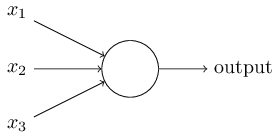
\includegraphics[width=0.9\textwidth]{images/tikz0.png}
\end{center}

\noindent 在所示的例子中，感知机有三个输入，$x_1, x_2, x_3$. 一般来说，它可能有更多或更少的输入.Rosenblatt 提出了一个简单的规则来计算输出. 他引入了权重\label{term:14}，$w_1,w_2,\ldots$，即表示各个输入对输出的重要性的实数. 神经元的输出，$0$ 或 $1$，取决于加权和 $\sum_j w_j x_j$ 是小于还是大于某个阈值\label{term:15}. 就像权重一样，阈值是一个实数，是神经元的一个参数. 用更精确的代数术语来说：

\begin{equation}
\mbox{output} = \left\{ \begin{array}{ll} 0 & \mbox{if } \sum_j w_j x_j \leq \mbox{ threshold} \\ 1 & \mbox{if } \sum_j w_j x_j > \mbox{ threshold} \end{array} \right.
\tag{1}
\end{equation}

\noindent 感知机的工作原理就是如此！

这就是基本的数学模型. 你可以把感知机看作是一种通过权衡证据来做出决策的设备. 让我举个例子. 这不是一个非常现实的例子，但它很容易理解，我们很快就会讲到更现实的例子. 假设周末快到了，你听说你的城市将举办一个奶酪节. 你喜欢奶酪，正在决定是否去参加这个节日. 你可能会通过权衡三个因素来做出决定：

\begin{enumerate}

\item 天气好吗？

\item 你的男朋友或女朋友想陪你吗？

\item 节日地点靠近公共交通吗？（你没有车）.

\end{enumerate}

我们可以用相应的二进制变量 $x_1, x_2$ 和 $x_3$ 来表示这三个因素. 例如，如果天气好，我们有 $x_1 = 1$，如果天气不好，$x_1 = 0$. 类似地，如果你的男朋友或女朋友想去，$x_2 = 1$，如果不想，$x_2 = 0$. 对于 $x_3$ 和公共交通也是如此.

现在，假设你非常喜欢奶酪，以至于即使你的男朋友或女朋友不感兴趣，而且节日地点很难到达，你也乐意去参加. 但也许你真的很讨厌坏天气，如果天气不好，你绝不会去参加节日. 你可以使用感知机来模拟这种决策. 一种方法是选择天气的权重 $w_1 = 6$，其他条件的权重 $w_2 = 2$ 和 $w_3 = 2$.$w_1$ 的较大值表明天气对你来说很重要，远比你男朋友或女朋友是否陪你，或公共交通是否近便更重要. 最后，假设你为感知机选择了阈值 $5$. 有了这些选择，感知机实现了所需的决策模型，每当天气好时输出 $1$，每当天气不好时输出 $0$. 你的男朋友或女朋友是否想去，或者公共交通是否在附近，对输出没有影响.

通过改变权重和阈值，我们可以得到不同的决策模型. 例如，假设我们改为选择阈值 $3$. 那么感知机将决定，只要天气好\emph{或}节日地点靠近公共交通\emph{且}你的男朋友或女朋友愿意陪你，你就应该去参加节日. 换句话说，这将是一个不同的决策模型. 降低阈值意味着你更愿意去参加节日.

显然，感知机并不是人类决策的完整模型！但这个例子说明的是感知机如何权衡不同种类的证据来做出决策. 而且，一个由感知机组成的复杂网络可以做出相当微妙的决策，这似乎是合理的：

\begin{center}
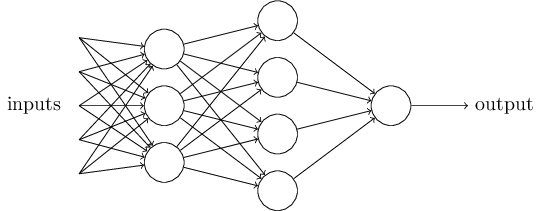
\includegraphics[width=0.9\textwidth]{images/tikz1.png}
\end{center}

\noindent 在这个网络中，第一列感知机——我们将称之为第一层感知机——通过权衡输入证据做出三个非常简单的决策. 第二层的感知机呢？这些感知机中的每一个都通过权衡第一层决策的结果来做出决策. 这样，第二层的感知机可以在比第一层感知机更复杂、更抽象的层次上做出决策. 而第三层的感知机可以做出更复杂的决策. 通过这种方式，一个多层的感知机网络可以进行复杂的决策.

顺便提一下，当我定义感知机时，我说感知机只有一个输出. 在上面的网络中，感知机看起来有多个输出. 事实上，它们仍然是单输出. 多个输出箭头仅仅是一种有用的方式，用来表示一个感知机的输出被用作其他几个感知机的输入. 这比画一条单一的输出线然后分叉要不那么笨拙.

让我们简化描述感知机的方式. 条件 $\sum_j w_j x_j > \mbox{threshold}$ 很繁琐，我们可以做两个符号上的改变来简化它. 第一个改变是将 $\sum_j w_j x_j$ 写成点积\label{term:16}，$w \cdot x \equiv \sum_j w_j x_j$，其中 $w$ 和 $x$ 是向量，其分量分别是权重和输入. 第二个改变是将阈值移到不等式的另一边，并用所谓的感知机的\emph{偏置}（bias）\label{term:5}代替它，$b \equiv -\mbox{threshold}$. 使用偏置代替阈值，感知机规则可以重写为：

\begin{equation}
\mbox{output} = \left\{ \begin{array}{ll} 0 & \mbox{if } w\cdot x + b \leq 0 \\ 1 & \mbox{if } w\cdot x + b > 0 \end{array} \right.
\tag{2}
\end{equation}

\noindent 你可以把偏置看作衡量让感知机输出 $1$ 有多容易的度量. 或者用更生物学的术语来说，偏置是衡量让感知机\emph{激发}有多容易的度量. 对于一个偏置非常大的感知机，它极容易输出 $1$. 但如果偏置非常负，那么感知机就很难输出 $1$. 显然，引入偏置只是我们描述感知机方式的一个小改变，但我们稍后会看到，它带来了进一步的符号简化. 因此，在本书的剩余部分，我们将不使用阈值，而是始终使用偏置.

我已经将感知机描述为一种权衡证据以做出决策的方法. 感知机的另一种用途是计算我们通常认为构成计算基础的基本逻辑函数，例如 \texttt{AND}、\texttt{OR} 和 \texttt{NAND}. 例如，假设我们有一个感知机，有两个输入，每个输入的权重为 $-2$，总偏置为 $3$. 这是我们的感知机：

\begin{center}
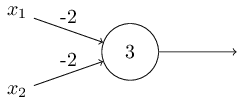
\includegraphics[width=0.9\textwidth]{images/tikz2.png}
\end{center}

\noindent 然后我们看到输入 $00$ 产生输出 $1$，因为 $(-2)*0+(-2)*0+3 = 3$ 是正的. 这里，我引入了 $*$ 符号来使乘法明确. 类似的计算表明，输入 $01$ 和 $10$ 产生输出 $1$. 但输入 $11$ 产生输出 $0$，因为 $(-2)*1+(-2)*1+3 = -1$ 是负的. 因此我们的感知机实现了一个 NAND 门！

\texttt{NAND} 的例子表明，我们可以使用感知机来计算简单的逻辑函数. 事实上，我们可以使用感知机网络来计算\emph{任何}逻辑函数. 原因是 \texttt{NAND} 门对于计算是通用的，也就是说，我们可以用 \texttt{NAND} 门构建任何计算. 例如，我们可以使用 \texttt{NAND} 门构建一个将两个比特 $x_1$ 和 $x_2$ 相加的电路. 这需要计算按位和 $x_1 \oplus x_2$，以及一个进位比特，当 $x_1$ 和 $x_2$ 都为 $1$ 时，该进位比特被设置为 $1$，即进位比特就是按位乘积 $x_1 x_2$：

\begin{center}
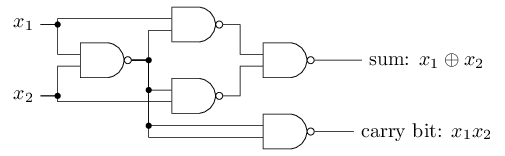
\includegraphics[width=0.9\textwidth]{images/tikz3.png}
\end{center}

\noindent 为了得到等效的感知机网络，我们将所有 NAND 门替换为具有两个输入的感知机，每个输入的权重为 $-2$，总偏置为 $3$. 这是得到的网络. 注意，我将对应于右下角 NAND 门的感知机稍微移动了一下，只是为了更容易在图上画箭头：

\begin{center}
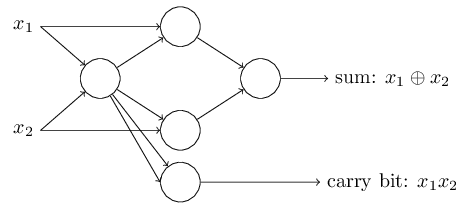
\includegraphics[width=0.9\textwidth]{images/tikz4.png}
\end{center}

\noindent 这个感知机网络的一个显著特点是，最左边感知机的输出被两次用作最底部感知机的输入. 当我定义感知机模型时，我没有说是否允许这种同一位置的双重输出. 实际上，这并不太重要. 如果我们不想允许这种事情，那么可以简单地将两条线合并为一条权重为 -4 的单一连接，而不是两条权重为 -2 的连接.（如果你觉得这不明显，你应该停下来向自己证明这是等价的.）有了这个改变，网络看起来如下，所有未标记的权重等于 -2，所有偏置等于 3，以及一个标记为 -4 的单一权重：

\begin{center}
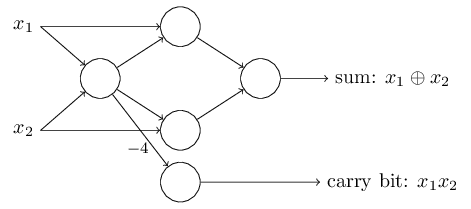
\includegraphics[width=0.9\textwidth]{images/tikz5.png}
\end{center}

\noindent 到目前为止，我一直将像 $x_1$ 和 $x_2$ 这样的输入画成漂浮在感知机网络左侧的变量. 事实上，按照惯例，我们会画一个额外的感知机层——输入层\label{term:17}——来编码输入：

\begin{center}
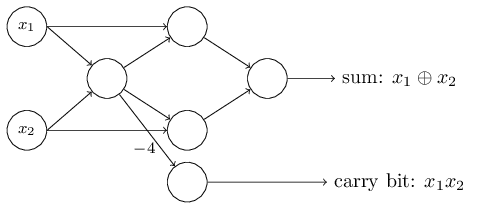
\includegraphics[width=0.9\textwidth]{images/tikz6.png}
\end{center}

\noindent 这种输入感知机的表示法，其中我们有一个输出，但没有输入，

\begin{center}
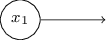
\includegraphics[width=0.9\textwidth]{images/tikz7.png}
\end{center}

\noindent 是一种简写. 它实际上并不意味着一个没有输入的感知机. 要看到这一点，假设我们确实有一个没有输入的感知机. 那么加权和 $\sum_j w_j x_j$ 将始终为零，因此如果 $b > 0$，感知机将输出 $1$，如果 $b \leq 0$，则输出 $0$. 也就是说，感知机将简单地输出一个固定值，而不是所需的值（在上面的例子中是 $x_1$）. 最好将输入感知机视为实际上根本不是感知机，而是特殊单元，它们被简单地定义为输出所需的值，$x_1, x_2,\ldots$.

加法器例子展示了如何使用感知机网络来模拟包含许多 \texttt{NAND} 门的电路. 而且因为 \texttt{NAND} 门对于计算是通用的，所以感知机对于计算也是通用的.

感知机的计算通用性既令人安心又令人失望. 它令人安心，因为它告诉我们感知机网络可以像任何其他计算设备一样强大. 但它也令人失望，因为它让人觉得感知机仅仅是一种新型的 \texttt{NAND} 门. 这算不上什么大新闻！

然而，情况比这种观点所暗示的要好. 事实证明，我们可以设计\emph{学习算法}，它可以自动调整人工神经元网络的权重和偏置. 这种调整是在响应外部刺激时发生的，没有程序员的直接干预. 这些学习算法使我们能够以一种与常规逻辑门截然不同的方式使用人工神经元. 我们的神经网络可以简单地学习解决问题，而不是明确地布置 \texttt{NAND} 和其他门的电路，有时这些问题直接设计常规电路会极其困难.
\sectionTitle{S 型神经元}{S 型神经元}

学习算法听起来很棒. 但我们如何为神经网络设计这样的算法呢？假设我们有一个感知机网络，想用它来学习解决某个问题. 例如，网络的输入可能是扫描的手写数字图像的原始像素数据. 我们希望网络学习权重和偏置，使得网络的输出能正确分类该数字. 为了了解学习可能如何工作，假设我们对网络中的某个权重（或偏置）做一个微小的改变. 我们希望的是，权重的这个微小改变只会引起网络输出的一个微小相应改变. 正如我们稍后将看到的，这一性质将使学习成为可能. 示意性地，这就是我们想要的（显然这个网络太简单，无法进行手写数字识别！）：

\begin{center}
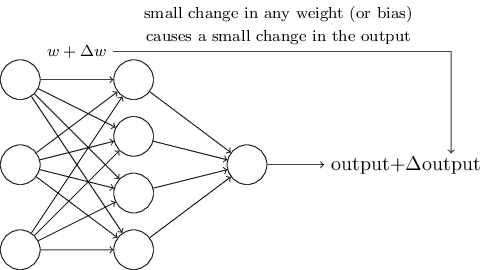
\includegraphics[width=0.9\textwidth]{images/tikz8.png}
\end{center}

\noindent 如果权重（或偏置）的微小改变只会引起输出的微小改变，那么我们就可以利用这一事实来修改权重和偏置，使网络的行为更符合我们的期望. 例如，假设网络错误地将一张图像分类为 ``8''，而它应该是 ``9''. 我们可以找出如何对权重和偏置做微小改变，使网络稍微更接近将图像分类为 ``9''. 然后我们重复这一过程，一次又一次地改变权重和偏置，以产生越来越好的输出. 网络就在学习了.

问题在于，当我们的网络包含感知机时，情况并非如此. 事实上，网络中任何单个感知机的权重或偏置的微小改变，有时会导致该感知机的输出完全翻转，比如从 $0$ 变为 $1$. 这种翻转随后可能导致网络其余部分的行为以某种非常复杂的方式完全改变. 因此，虽然你的 ``9'' 现在可能被正确分类了，但网络在所有其他图像上的行为很可能已经以某种难以控制的方式完全改变了. 这使得我们很难看到如何逐步修改权重和偏置，使网络更接近期望的行为. 也许有某种巧妙的方法可以绕过这个问题. 但如何让感知机网络学习并不是显而易见的.

我们可以通过引入一种新类型的人工神经元来克服这个问题，称为 S 型神经元. S 型神经元与感知机类似，但经过修改，使其权重和偏置的微小改变只会引起输出的微小改变. 这是关键事实，它将使 S 型神经元网络能够学习.

好的，让我来描述 S 型神经元. 我们将用与描述感知机相同的方式来描绘 S 型神经元：

\begin{center}
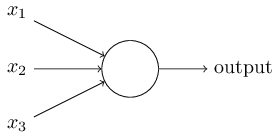
\includegraphics[width=0.9\textwidth]{images/tikz9.png}
\end{center}

\noindent 就像感知机一样，S 型神经元有输入，$x_1, x_2, \ldots$. 但这些输入不只是 $0$ 或 $1$，还可以取 $0$ 到 $1$ 之间的任意值. 例如，$0.638\ldots$ 是 S 型神经元的有效输入. 同样像感知机一样，S 型神经元对每个输入都有权重，$w_1, w_2, \ldots$，以及一个总偏置，$b$. 但输出不是 $0$ 或 $1$. 相反，它是 $\sigma(w \cdot x+b)$，其中 $\sigma$ 被称为 S 型函数\label{term:18} * *顺便说一句，$\sigma$ 有时被称为逻辑斯蒂函数\label{term:19}，这类新神经元被称为逻辑斯蒂神经元. 记住这个术语很有用，因为许多从事神经网络工作的人都使用这些术语. 不过，我们将坚持使用 S 型这一术语.，其定义为：

\begin{equation}
\sigma(z) \equiv \frac{1}{1+e^{-z}}.
\tag{3}
\end{equation}

\noindent 更明确地说，一个 S 型神经元在输入为 $x_1,x_2,\ldots$、权重为 $w_1,w_2,\ldots$、偏置为 $b$ 时的输出是

\begin{equation}
\frac{1}{1+\exp(-\sum_j w_j x_j-b)}.
\tag{4}
\end{equation}

\noindent 乍一看，S 型神经元与感知机看起来非常不同. 如果你还不熟悉 S 型函数，它的代数形式可能显得晦涩难懂. 事实上，感知机和 S 型神经元之间有许多相似之处，而 S 型函数的代数形式更多地是一个技术细节，而不是理解上的真正障碍.

为了理解与感知机模型的相似性，假设 $z \equiv w \cdot x + b$ 是一个很大的正数. 那么 $e^{-z} \approx 0$，因此 $\sigma(z) \approx 1$. 换句话说，当 $z = w \cdot x+b$ 很大且为正时，S 型神经元的输出近似为 $1$，就像感知机一样. 另一方面，假设 $z = w \cdot x+b$ 非常负. 那么 $e^{-z} \rightarrow \infty$，且 $\sigma(z) \approx 0$. 所以当 $z = w \cdot x +b$ 非常负时，S 型神经元的行为也密切近似于感知机. 只有当 $w \cdot x+b$ 的大小适中时，才会与感知机模型有较大偏差.

那么 $\sigma$ 的代数形式呢？我们如何理解它？事实上，$\sigma$ 的确切形式并不那么重要——真正重要的是函数绘制出来的形状. 形状如下：这个形状是阶梯函数平滑化后的版本：如果 $\sigma$ 实际上是一个阶梯函数，那么 S 型神经元就 \emph{是} 一个感知机，因为输出将是 $1$ 或 $0$，取决于 $w\cdot x+b$ 是正还是负*\footnote{实际上，当 $w \cdot x +b = 0$ 时，感知机输出 $0$，而阶梯函数输出 $1$. 所以严格来说，我们需要在那一点修改阶梯函数. 但你明白意思了.}. 通过使用实际的 $\sigma$ 函数，我们得到的是，如上文已经暗示的，一个平滑化的感知机. 事实上，正是 $\sigma$ 函数的平滑性才是关键事实，而不是它的具体形式. $\sigma$ 的平滑性意味着权重中的微小变化 $\Delta w_j$ 和偏置中的微小变化 $\Delta b$ 将产生神经元输出的微小变化 $\Delta \mbox{output}$. 事实上，微积分告诉我们 $\Delta \mbox{output}$ 可以很好地近似为

\begin{equation}
\Delta \mbox{output} \approx \sum_j \frac{\partial \, \mbox{output}}{\partial w_j} \Delta w_j + \frac{\partial \, \mbox{output}}{\partial b} \Delta b,
\tag{5}
\end{equation}

\noindent 其中求和是对所有
权重 $w_j$ 进行的，$\partial \, \mbox{output} / \partial w_j$ 和 $\partial \, \mbox{output} /\partial b$ 分别表示 $\mbox{output}$ 对 $w_j$ 和 $b$ 的偏导数\label{term:21}\label{term:20}. 如果你对偏导数不太熟悉，不要慌张！虽然上面的表达式看起来很复杂，有那么多偏导数，但它实际上说的是一件非常简单的事（而且是非常好的消息）：$\Delta \mbox{output}$ 是权重和偏置的变化 $\Delta w_j$ 和 $\Delta b$ 的 \emph{线性函数}. 这种线性关系使得我们可以很容易地选择权重和偏置的微小变化，以实现输出中任何期望的微小变化. 因此，虽然 S 型神经元在定性行为上与感知机有许多相同之处，但它们使我们更容易弄清楚改变权重和偏置将如何改变输出.

如果真正重要的是 $\sigma$ 的形状，而不是它的确切形式，那么为什么要使用方程 (3) 中 $\sigma$ 所用的特定形式

\begin{align*}
\sigma(z) \equiv \frac{1}{1+e^{-z}} \nonumber
\end{align*}

\noindent 呢？事实上，在本书后面，我们偶尔会考虑输出为 $f(w \cdot x + b)$ 的神经元，其中 $f(\cdot)$ 是某种其他的 \emph{激活函数}. 当我们使用不同的激活函数时，主要的变化是方程 (5) 中偏导数的具体值

\begin{align*}
\Delta \mbox{output} \approx \sum_j \frac{\partial \, \mbox{output}}{\partial w_j} \Delta w_j + \frac{\partial \, \mbox{output}}{\partial b} \Delta b \nonumber
\end{align*}

\noindent 会改变. 事实证明，当我们稍后计算这些偏导数时，使用 $\sigma$ 将简化代数运算，这仅仅是因为指数函数在微分时具有优美的性质. 无论如何，$\sigma$ 在神经网络研究中被广泛使用，并且是我们在本书中最常使用的激活函数\label{term:22}.

我们应该如何解释 S 型神经元的输出？显然，感知机和 S 型神经元之间的一个重大区别是，S 型神经元不只输出 $0$ 或 $1$. 它们可以输出 $0$ 到 $1$ 之间的任何实数，因此像 $0.173\ldots$ 和 $0.689\ldots$ 这样的值都是合法的输出. 这可能很有用，例如，如果我们想用输出值来表示输入到神经网络的图像中像素的平均强度. 但有时它也可能带来麻烦. 假设我们希望网络的输出表明 ``输入图像是 9'' 或 ``输入图像不是 9''. 显然，如果输出是 $0$ 或 $1$，就像感知机那样，做这件事会最容易. 但在实践中，我们可以建立一个约定来处理这个问题，例如，决定将任何至少为 $0.5$ 的输出解释为表示 ``9''，而将任何小于 $0.5$ 的输出解释为表示 ``不是 9''. 当我们使用这样的约定时，我总会明确说明，因此它不应该引起任何混淆.

\begin{exerciseBox}{练习}

\begin{itemize}

\item \textbf{模拟感知机的 S 型神经元，第一部分} $\mbox{}$ \\ 假设我们取一个感知机网络中的所有
权重和偏置，并将它们乘以一个正常数 $c > 0$. 证明网络的行为不变.

\item \textbf{模拟感知机的 S 型神经元，第二部分} $\mbox{}$ \\ 假设我们有与上一题相同的设置——一个感知机网络. 还假设感知机网络的整体输入已经选定. 我们不需要实际的输入值，只需要输入已经固定. 假设权重和偏置使得对于网络中任何特定感知机的输入 $x$，都有 $w \cdot x + b \neq 0$. 现在将网络中的所有感知机替换为 S 型神经元，并将权重和偏置乘以一个正常数 $c > 0$. 证明当 $c \rightarrow \infty$ 时，这个 S 型神经元网络的行为与感知机网络完全相同. 当其中一个感知机满足 $w \cdot x + b = 0$ 时，这为什么会失效？

\end{itemize}

\end{exerciseBox}
\sectionTitle{神经网络的结构}{神经网络的结构}

在下一节中，我将介绍一个能够相当出色地分类手写数字的神经网络. 为了做好准备，先解释一些术语会有所帮助，这些术语让我们能够命名网络的不同部分. 假设我们有这样一个网络：

\begin{center}
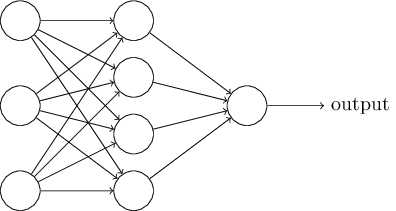
\includegraphics[width=0.9\textwidth]{images/tikz10.png}
\end{center}

\noindent 如前所述，这个网络中最左边的一层称为输入层，该层内的神经元称为输入神经元. 最右边的一层，即输出层\label{term:23}，包含输出神经元，或者像本例中那样，只包含一个输出神经元. 中间层称为隐藏层\label{term:24}，因为这一层中的神经元既不是输入也不是输出. ``隐藏''这个词听起来可能有点神秘——我第一次听到这个词时，以为它一定有什么深刻的哲学或数学意义——但它实际上只不过意味着``既不是输入也不是输出''. 上面的网络只有一个隐藏层，但有些网络有多个隐藏层. 例如，下面这个四层网络有两个隐藏层：

\begin{center}
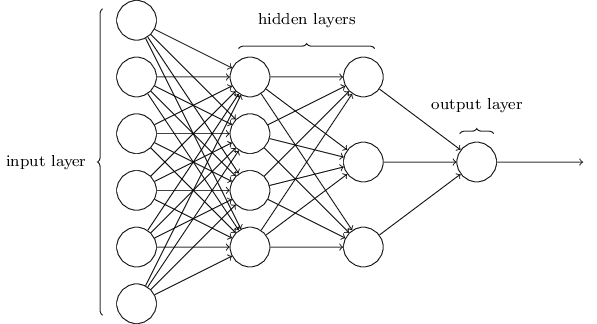
\includegraphics[width=0.9\textwidth]{images/tikz11.png}
\end{center}

\noindent 有点令人困惑的是，由于历史原因，这种多层网络有时被称为多层感知机或 MLP，尽管它们是由 S 型神经元而非感知机构成的. 我在这本书中不会使用 MLP 这个术语，因为我认为它容易引起混淆，但想提醒你它的存在.

网络中输入层和输出层的设计通常很直接. 例如，假设我们要判断一张手写图像是否描绘了一个``9''. 设计网络的一种自然方式是将图像像素的强度编码到输入神经元中. 如果图像是一张 $64$ 乘 $64$ 的灰度图像，那么我们会有 $4,096 = 64 \times 64$ 个输入神经元，其强度被适当地缩放到 $0$ 和 $1$ 之间. 输出层将只包含一个神经元，输出值小于 $0.5$ 表示``输入图像不是 9''，大于 $0.5$ 表示``输入图像是 9''.

虽然神经网络的输入层和输出层的设计通常很直接，但隐藏层的设计却可能相当有艺术性. 特别是，无法用几条简单的经验法则来概括隐藏层的设计过程. 相反，神经网络研究人员已经为隐藏层发展出了许多设计启发式方法，这些方法帮助人们从他们的网络中获得想要的行为. 例如，这类启发式方法可以用来帮助确定如何在隐藏层的数量和训练网络所需的时间之间进行权衡. 我们将在本书后面遇到几种这样的设计启发式方法.

到目前为止，我们讨论的都是这样一类神经网络：其中一层的输出被用作下一层的输入. 这样的网络被称为\emph{前馈}神经网络. 这意味着网络中没有环路——信息总是向前馈送，从不向后反馈. 如果我们确实有环路，就会出现 $\sigma$ 函数的输入依赖于输出的情况. 那将很难理解，所以我们不允许这样的环路.

然而，还有其他类型的人工神经网络模型，其中反馈环路是可能的. 这些模型被称为循环神经网络\label{term:25}. 这些模型中的想法是让神经元在有限的一段时间内激活，然后进入静息状态. 这种激活可以刺激其他神经元，这些神经元可能稍后也会激活一段时间. 这又会导致更多的神经元激活，因此随着时间的推移，我们会得到一连串激活的神经元. 在这样的模型中，环路不会引起问题，因为一个神经元的输出只会在稍后的时间影响其输入，而不是瞬时影响.

循环神经网络的影响力不如前馈\label{term:26}网络，部分原因是循环网络的学习算法（至少到目前为止）不够强大. 但循环网络仍然极其有趣. 它们在精神上比前馈网络更接近我们大脑的工作方式. 而且循环网络有可能解决那些前馈网络极难解决的重要问题. 然而，为了限制我们的范围，在本书中我们将集中讨论使用更广泛的前馈网络.
\sectionTitle{一个识别手写数字的简单网络}{一个识别手写数字的简单网络}

定义了神经网络之后，让我们回到手写数字识别. 我们可以把识别手写数字的问题拆分成两个子问题. 首先，我们需要一种方法，把一张包含多个数字的图像拆分成一系列单独的图像，每张图像只包含一个数字. 例如，我们希望把图像

\begin{center}
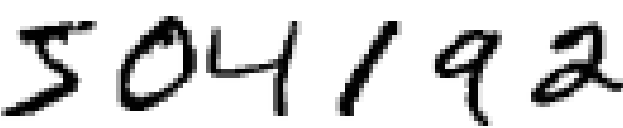
\includegraphics[width=0.500\textwidth]{images/digits.png}
\end{center}

\noindent 拆分成六张单独的图像，

\begin{center}
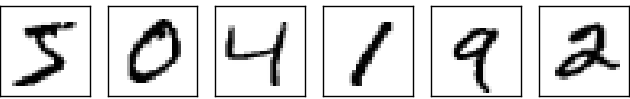
\includegraphics[width=0.733\textwidth]{images/digits_separate.png}
\end{center}

\noindent 我们人类可以轻松地解决这个\emph{分割问题}（segmentation problem）\label{term:6}，但对计算机程序来说，正确地拆分图像却颇具挑战性. 一旦图像被分割开，程序就需要对每个单独的数字进行分类. 例如，我们希望程序能够识别出上面第一张图像

\begin{center}
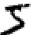
\includegraphics[width=0.107\textwidth]{images/mnist_first_digit.png}
\end{center}

\noindent 是一个 5.

我们将专注于编写一个程序来解决第二个问题，也就是对单个数字进行分类. 我们这样做是因为，一旦你有了对单个数字进行分类的好方法，分割问题其实并不那么难解决. 解决分割问题有很多方法. 一种方法是尝试许多不同的图像分割方式，用单个数字分类器为每种尝试的分割打分. 如果单个数字分类器对各个分割段中的分类都很有信心，那么这种尝试的分割就得到高分；如果分类器在一个或多个分割段中遇到很大困难，那么就得到低分. 其想法是，如果分类器在某处遇到困难，那么很可能是因为分割方式选择得不正确. 这个想法以及其他变体可以用来相当好地解决分割问题. 所以，与其操心分割问题，我们不如集中精力开发一个神经网络，来解决更有趣也更困难的问题，即识别单个手写数字.

为了识别单个数字，我们将使用一个三层神经网络：

\begin{center}
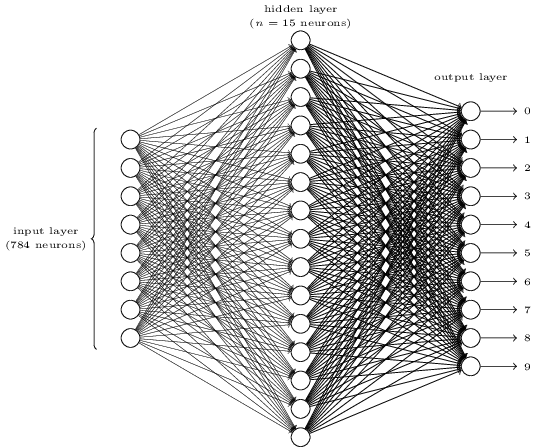
\includegraphics[width=0.9\textwidth]{images/tikz12.png}
\end{center}

\noindent 网络的输入层包含对输入像素值进行编码的神经元. 正如下一节将要讨论的，我们用于训练网络的数据将由许多 $28$ 乘 $28$ 像素的扫描手写数字图像组成，因此输入层包含 $784 = 28 \times 28$ 个神经元. 为简单起见，我在上图中省略了 $784$ 个输入神经元中的大部分. 输入像素是灰度的，值 $0.0$ 表示白色，值 $1.0$ 表示黑色，介于两者之间的值表示逐渐变暗的灰色.

网络的第二层是一个隐藏层. 我们用 $n$ 表示这个隐藏层中神经元的数量，并将尝试不同的 $n$ 值. 图中所示的例子展示了一个很小的隐藏层，只包含 $n = 15$ 个神经元.

网络的输出层包含 10 个神经元. 如果第一个神经元激活，即输出 $\approx 1$，那么这表明网络认为该数字是 $0$. 如果第二个神经元激活，那么这表明网络认为该数字是 $1$. 依此类推. 更精确一点说，我们把输出神经元从 $0$ 到 $9$ 编号，然后找出哪个神经元的激活值\label{term:27}最高. 如果那个神经元是，比如说，编号为 $6$ 的神经元，那么我们的网络就会猜测输入的数字是 $6$. 对其他输出神经元也依此类推.

你可能会想，为什么我们要使用 $10$ 个输出神经元. 毕竟，网络的目标是告诉我们输入图像对应哪个数字（$0, 1, 2, \ldots, 9$）. 一种看似自然的方式是只使用 $4$ 个输出神经元，把每个神经元看作取一个二值，取决于该神经元的输出更接近 $0$ 还是更接近 $1$. 四个神经元足以编码答案，因为 $2^4 = 16$ 大于输入数字的 10 个可能取值. 为什么我们的网络反而要使用 $10$ 个神经元呢？这不是很低效吗？最终的理由是经验性的：我们可以把两种网络设计都试一下，结果发现，对于这个特定的问题，使用 $10$ 个输出神经元的网络比使用 $4$ 个输出神经元的网络学得更好. 但这让我们不禁想问，\emph{为什么}使用 $10$ 个输出神经元效果更好. 有没有某种启发式方法能事先告诉我们，应该使用 $10$ 输出的编码而不是 $4$ 输出的编码？

要理解我们为什么这样做，从基本原理出发思考神经网络在做什么会有所帮助. 先考虑我们使用 $10$ 个输出神经元的情况. 让我们把注意力集中在第一个输出神经元上，也就是那个试图判断数字是不是 $0$ 的神经元. 它通过权衡来自隐藏层神经元的证据来做到这一点. 那些隐藏神经元在做什么呢？好吧，不妨为了讨论起见假设隐藏层中的第一个神经元检测如下图像是否存在：

\begin{center}
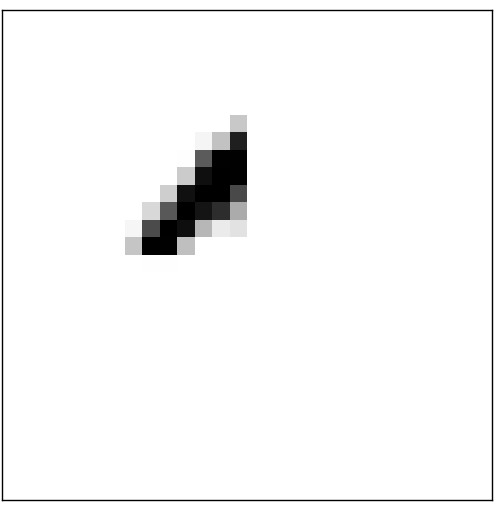
\includegraphics[width=0.217\textwidth]{images/mnist_top_left_feature.png}
\end{center}

\noindent 它可以通过给与该图像重叠的输入像素赋予很大的权重，而只给其他输入赋予很小的权重来做到这一点. 类似地，不妨为了讨论起见假设隐藏层中的第二、第三和第四个神经元检测如下图像是否存在：

\begin{center}
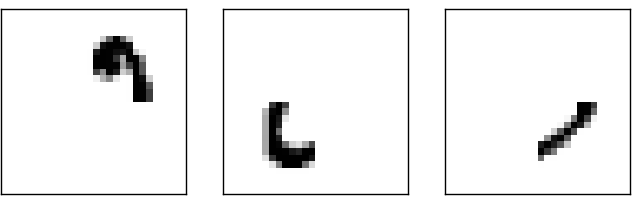
\includegraphics[width=0.707\textwidth]{images/mnist_other_features.png}
\end{center}

\noindent 你可能已经猜到了，这四张图像合在一起就构成了我们之前在那行数字中看到的 $0$ 图像：

\begin{center}
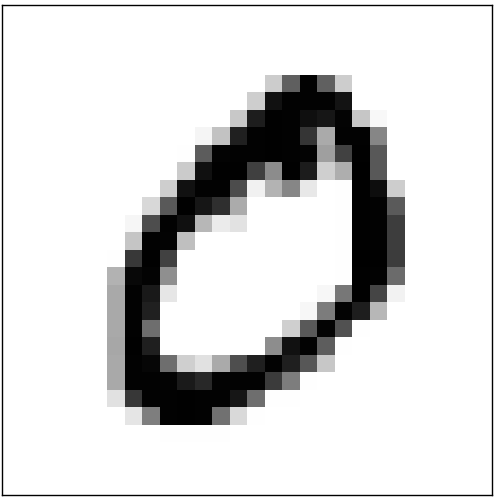
\includegraphics[width=0.217\textwidth]{images/mnist_complete_zero.png}
\end{center}

\noindent 所以，如果这四个隐藏神经元都激活，那么我们就可以得出结论：该数字是 $0$. 当然，这并不是我们用来断定图像是 $0$ 的\emph{唯一}证据 - 我们还可以通过许多其他方式合理地得到 $0$（比如，通过上述图像的平移，或轻微的变形）. 但至少在这个例子中，我们可以有把握地说，我们会断定输入是 $0$.

假设神经网络以这种方式运作，我们就能为为什么网络有 $10$ 个输出比有 $4$ 个输出更好给出一个合理的解释. 如果我们有 $4$ 个输出，那么第一个输出神经元将试图判断该数字的最高有效位是什么. 而要把那个最高有效位与上面所示的简单形状联系起来，并没有容易的办法. 很难想象数字的组成形状会与（比如说）输出中的最高有效位有任何好的历史性关联.

话虽如此，这一切都只是一种启发式. 没有什么规定说三层神经网络必须按我描述的方式运作，让隐藏神经元检测简单的组成形状. 也许某个聪明的学习算法会找到某种权重分配，让我们只使用 $4$ 个输出神经元. 但作为一种启发式，我所描述的这种思考方式相当有效，并且可以在设计好的神经网络结构时为你节省大量时间.

\begin{exerciseBox}{练习}

\begin{itemize}

\item 有一种方法可以通过在上面的三层网络中增加一个额外的层来确定数字的按位表示. 这个额外的层把前一层的输出转换成二进制表示，如下图所示. 为新的输出层找出一组权重和偏置. 假设前 $3$ 层神经元使得第三层（即旧的输出层）中正确输出的激活值至少为 $0.99$，而不正确输出的激活值小于 $0.01$.

\end{itemize}

\begin{center}
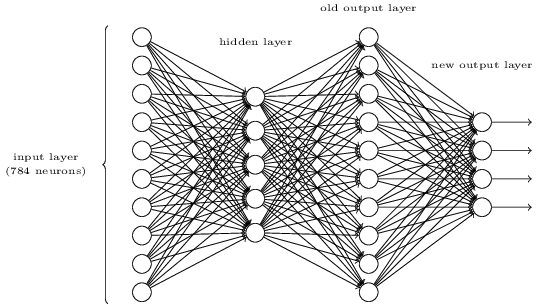
\includegraphics[width=0.9\textwidth]{images/tikz13.png}
\end{center}

\end{exerciseBox}
\sectionTitle{用梯度下降进行学习}{用梯度下降进行学习}

现在我们已经为神经网络设计好了结构，它如何学习识别数字呢？我们首先需要的是一个用于学习的数据集——即所谓的训练数据\label{term:28}集. 我们将使用 MNIST 数据集，其中包含数万张手写数字的扫描图像，以及它们正确的分类.MNIST 这个名字来源于它是 NIST（美国国家标准与技术研究院）收集的两个数据集的修改子集. 下面是 MNIST 中的几张图像：

\begin{center}
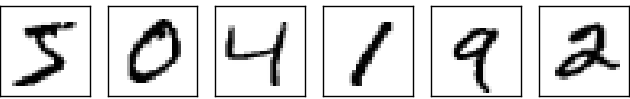
\includegraphics[width=0.700\textwidth]{images/digits_separate.png}
\end{center}

\noindent 如你所见，这些数字实际上与本章开头作为识别挑战展示的那些数字相同. 当然，在测试我们的网络时，我们会让它识别不在训练集\label{term:29}中的图像！

MNIST 数据分为两部分. 第一部分包含 60,000 张图像，用作训练数据. 这些图像是来自 250 人的手写样本扫描件，其中一半是美国人口普查局的员工，一半是高中生. 图像是灰度的，大小为 28 乘 28 像素.MNIST 数据集的第二部分是 10,000 张图像，用作测试数据\label{term:30}. 同样，这些是 28 乘 28 的灰度图像. 我们将使用测试数据来评估我们的神经网络学习识别数字的效果. 为了使其成为对性能的良好测试，测试数据取自与原始训练数据\emph{不同}的 250 人（尽管仍然是在人口普查局员工和高中生之间划分的群体）. 这有助于让我们相信，我们的系统能够识别那些在训练期间未见过其笔迹的人所写的数字.

我们将使用符号 $x$ 来表示一个训练输入. 将每个训练输入 $x$ 视为一个 $28 \times 28 = 784$ 维向量\label{term:31}会很方便. 向量中的每个条目代表图像中单个像素的灰度值. 我们将相应的期望输出记为 $y = y(x)$，其中 $y$ 是一个 $10$ 维向量. 例如，如果某个特定的训练图像 $x$ 描绘的是 $6$，那么 $y(x) = (0, 0, 0, 0, 0, 0, 1, 0, 0, 0)^T$ 就是网络期望的输出. 注意这里的 $T$ 是转置操作，将行向量转换为普通的（列）向量.

我们想要的是一个算法，它能让我们找到权重和偏置，使得对于所有训练输入 $x$，网络的输出都近似于 $y(x)$. 为了量化我们实现这一目标的程度，我们定义一个\emph{代价函数}*\footnote{有时也被称为\emph{损失}函数或\emph{目标}函数. 在本书中我们使用代价函数这一术语，但你应该注意其他术语，因为它们经常出现在研究论文和其他关于神经网络的讨论中.}：

\begin{equation}
C(w,b) \equiv \frac{1}{2n} \sum_x \| y(x) - a\|^2.
\tag{6}
\end{equation}

\noindent 这里，$w$ 表示网络中所有\emph{权重}的集合，$b$ 表示所有\emph{偏置}，$n$ 是训练输入的总数，$a$ 是当输入为 $x$ 时网络的输出向量，求和是对所有训练输入 $x$ 进行的. 当然，输出 $a$ 依赖于 $x$、$w$ 和 $b$，但为了保持符号简洁，我没有明确表示这种依赖关系. 符号 $\| v \|$ 只是表示向量 $v$ 的通常长度函数. 我们将 $C$ 称为\emph{二次}代价函数\label{term:32}；它有时也被称为\emph{均方误差}或简称 \emph{MSE}. 观察二次代价\label{term:33}函数的形式，我们看到 $C(w,b)$ 是非负的，因为求和中的每一项都是非负的. 此外，当对于所有训练输入 $x$，$y(x)$ 都近似等于输出 $a$ 时，代价 $C(w,b)$ 恰好变得很小，即 $C(w,b) \approx 0$. 因此，如果我们的训练算法\label{term:34}能够找到权重和偏置使得 $C(w,b) \approx 0$，那么它就做得很好. 相反，当 $C(w,b)$ 很大时，它就做得不太好——那意味着对于大量输入，$y(x)$ 并不接近输出 $a$. 因此，我们训练算法的目标将是最小化作为权重和偏置函数的代价 $C(w,b)$. 换句话说，我们想要找到一组使代价尽可能小的权重和偏置. 我们将使用一种称为\emph{梯度下降}的算法来实现这一点.

为什么要引入二次代价？毕竟，我们主要感兴趣的不是网络正确分类的图像数量吗？为什么不直接尝试最大化那个数量，而是最小化像二次代价这样的代理指标呢？问题在于，正确分类的图像数量并不是网络中权重和偏置的光滑函数. 在大多数情况下，对权重和偏置进行微小改变根本不会导致正确分类的训练图像数量发生任何变化. 这使得我们很难弄清楚如何改变权重和偏置来提高性能. 如果我们改用像二次代价这样的光滑代价函数，那么就容易弄清楚如何对权重和偏置进行微小改变，从而改善代价. 这就是为什么我们首先关注最小化二次代价，之后才会考察分类准确率.

即使我们想要使用光滑的代价函数，你可能仍然想知道为什么我们选择方程 (6) 中使用的二次函数

\begin{align*}
C(w,b) \equiv \frac{1}{2n} \sum_x \| y(x) - a\|^2 \nonumber
\end{align*}

\noindent. 这不是一个相当\emph{特设}的选择吗？也许如果我们选择不同的代价函数，我们会得到一组完全不同的最小化权重和偏置？这是一个合理的担忧，稍后我们会重新审视代价函数，并做一些修改. 然而，方程 (6) 中的二次代价函数

\begin{align*}
C(w,b) \equiv \frac{1}{2n} \sum_x \| y(x) - a\|^2 \nonumber
\end{align*}

\noindent 对于理解神经网络学习的基础知识来说完全够用，所以我们现在就坚持使用它.

回顾一下，我们训练神经网络的目标是找到使二次代价函数 $C(w, b)$ 最小化的权重和偏置. 这是一个适定问题，但就目前的形式而言，它有很多分散注意力的结构——将 $w$ 和 $b$ 解释为权重和偏置，背景中潜伏的 $\sigma$ 函数，网络结构的选择，MNIST，等等. 事实证明，通过忽略大部分这些结构，只专注于最小化方面，我们可以理解大量内容. 所以现在我们要忘记代价函数的具体形式、与神经网络的联系等等. 相反，我们将想象我们只是被给定了许多变量的一个函数，我们想要最小化那个函数. 我们将发展一种称为\emph{梯度下降}的技术，它可以用来解决这类最小化问题. 然后我们再回到我们想要为神经网络最小化的具体函数.

好的，假设我们试图最小化某个函数 $C(v)$. 这可以是许多变量的任何实值函数，$v = v_1, v_2, \ldots$. 注意我已经用 $v$ 替换了 $w$ 和 $b$ 的记号，以强调这可以是任何函数——我们不再特别在神经网络的背景下思考. 为了最小化 $C(v)$，将 $C$ 想象成仅有两个变量的函数会有所帮助，我们将这两个变量称为 $v_1$ 和 $v_2$：

\begin{center}
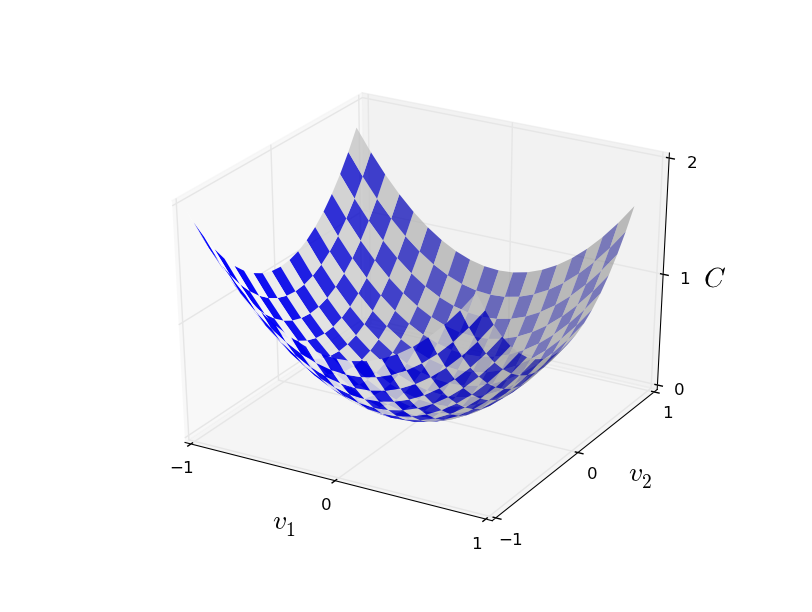
\includegraphics[width=0.903\textwidth]{images/valley.png}
\end{center}

\noindent 我们想要找到 $C$ 达到其全局最小值的位置. 当然，对于上面绘制的函数，我们可以目测图形并找到最小值. 从这个意义上说，我可能展示了一个稍微\emph{过于}简单的函数！一个一般的函数 $C$ 可能是许多变量的复杂函数，通常不可能仅仅通过目测图形来找到最小值.

解决这个问题的一种方法是使用微积分来尝试解析地找到最小值. 我们可以计算导数，然后尝试用它们来找到 $C$ 取极值的位置. 如果运气好的话，当 $C$ 只是一个或几个变量的函数时，这可能行得通. 但当我们有更多变量时，这将变成一场噩梦. 而对于神经网络，我们通常想要\emph{远}更多的变量——最大的神经网络的代价函数以极其复杂的方式依赖于数十亿的权重和偏置. 使用微积分来最小化那根本行不通！（在断言我们将通过将 $C$ 想象成仅有两个变量的函数来获得洞察力之后，我在两段话中两次转身说，“嘿，但如果它是远多于两个变量的函数呢？”对此我很抱歉. 请相信我，将 $C$ 想象成两个变量的函数确实有帮助. 只是有时那幅图景会失效，而最后两段话就是在处理这种失效. 好的数学思考往往涉及同时处理多个直观图景，学会何时适合使用每个图景，何时不适合.）

好的，所以微积分行不通. 幸运的是，有一个漂亮的类比暗示了一种效果相当好的算法. 我们首先将我们的函数想象成一种山谷. 如果你稍微眯眼看上面的图，那应该不难. 我们想象一个球沿着山谷的斜坡滚下. 我们的日常经验告诉我们，球最终会滚到谷底. 也许我们可以用这个想法作为找到函数最小值的方法？我们会随机选择一个（假想的）球的起点，然后模拟球滚到谷底的运动. 我们可以简单地通过计算 $C$ 的导数（也许还有一些二阶导数）来进行这种模拟——这些导数会告诉我们关于山谷局部“形状”所需的一切信息，从而告诉我们球应该如何滚动.

基于我刚才写的内容，你可能会认为我们将尝试写下球的牛顿运动方程，考虑摩擦和重力等的影响. 实际上，我们不会那么认真地对待滚球的类比——我们是在设计一种最小化 $C$ 的算法，而不是开发物理定律的精确模拟！球的视角是为了激发我们的想象力，而不是限制我们的思考. 所以，与其陷入物理学的所有混乱细节，不如简单地问自己：如果我们被宣布为一天的神，可以制定自己的物理定律，指示球应该如何滚动，我们可以选择什么运动定律，使得球总是滚到谷底？

为了使这个问题更精确，让我们思考一下当我们在 $v_1$ 方向上将球移动一小段 $\Delta v_1$，在 $v_2$ 方向上将球移动一小段 $\Delta v_2$ 时会发生什么. 微积分告诉我们 $C$ 的变化如下：

\begin{equation}
\Delta C \approx \frac{\partial C}{\partial v_1} \Delta v_1 + \frac{\partial C}{\partial v_2} \Delta v_2.
\tag{7}
\end{equation}

\noindent 我们将找到一种选择 $\Delta v_1$ 和 $\Delta v_2$ 的方法，使得 $\Delta C$ 为负；即，我们将选择它们使得球向谷底滚下. 为了弄清楚如何做出这样的选择，定义 $\Delta v$ 为 $v$ 中变化的向量会有所帮助，$\Delta v \equiv (\Delta v_1, \Delta v_2)^T$，其中 $T$ 同样是转置操作，将行向量转换为列向量. 我们还将 $C$ 的\emph{梯度}定义为偏导数的向量，$\left(\frac{\partial C}{\partial v_1}, \frac{\partial C}{\partial v_2}\right)^T$. 我们用 $\nabla C$ 表示梯度向量，即：

\begin{equation}
\nabla C \equiv \left( \frac{\partial C}{\partial v_1}, \frac{\partial C}{\partial v_2} \right)^T.
\tag{8}
\end{equation}

\noindent 稍后我们将用 $\Delta v$ 和梯度 $\nabla C$ 来重写变化 $\Delta C$. 但在那之前，我想澄清一些有时会让人对梯度感到困惑的事情. 当第一次遇到 $\nabla C$ 记号时，人们有时会想知道应该如何思考 $\nabla$ 符号.$\nabla$ 到底是什么意思？事实上，将 $\nabla C$ 视为一个单一的数学对象——上面定义的向量——是完全没问题的，它恰好用两个符号来书写. 从这个观点来看，$\nabla$ 只是一点记号上的旗帜挥舞，告诉你“嘿，$\nabla C$ 是一个梯度向量”. 还有更高级的观点，其中 $\nabla$ 可以被视为一个独立的数学实体（例如，作为一个微分算子），但我们不需要这样的观点.

有了这些定义，表达式 (7)
\begin{align*}
\Delta C \approx \frac{\partial C}{\partial v_1} \Delta v_1 + \frac{\partial C}{\partial v_2} \Delta v_2 \nonumber
\end{align*}

\noindent $\Delta C$ 可以改写为

\begin{equation}
\Delta C \approx \nabla C \cdot \Delta v.
\tag{9}
\end{equation}

\noindent 这个方程有助于解释为什么 $\nabla C$ 被称为梯度向量：$\nabla C$ 将 $v$ 的变化与 $C$ 的变化联系起来，正如我们对一个被称为梯度的东西所期望的那样. 但这个方程真正令人兴奋的地方在于，它让我们看到如何选择 $\Delta v$ 以使 $\Delta C$ 为负. 特别地，假设我们选择

\begin{equation}
\Delta v = -\eta \nabla C,
\tag{10}
\end{equation}

\noindent 其中 $\eta$ 是一个小的正参数（被称为\emph{学习率}）. 那么方程 (9)

\begin{align*}
\Delta C \approx \nabla C \cdot \Delta v \nonumber
\end{align*}

\noindent 告诉我们 $\Delta C \approx -\eta \nabla C \cdot \nabla C = -\eta \|\nabla C\|^2$. 因为 $\| \nabla C \|^2 \geq 0$，这保证了 $\Delta C \leq 0$，即如果我们按照 (10) 中的规定改变 $v$，$C$ 将始终减小，永不增大

\begin{align*}
\Delta v = -\eta \nabla C \nonumber
\end{align*}

\noindent. （当然，这是在方程 (9) 近似的限度内

\begin{align*}
\Delta C \approx \nabla C \cdot \Delta v \nonumber
\end{align*}

\noindent ）. 这正是我们想要的属性！因此我们将用方程 (10)

\begin{align*}
\Delta v = -\eta \nabla C \nonumber
\end{align*}

\noindent 来定义梯度下降算法中小球的``运动定律''. 也就是说，我们将使用方程 (10)

\begin{align*}
\Delta v = -\eta \nabla C \nonumber
\end{align*}

\noindent 来计算 $\Delta v$ 的值，然后将小球的位置 $v$ 移动该数量：

\begin{equation}
v \rightarrow v' = v -\eta \nabla C.
\tag{11}
\end{equation}

\noindent 然后我们再次使用这个更新规则，进行另一次移动. 如果我们一遍又一遍地这样做，我们将不断减小 $C$，直到——我们希望——达到一个全局最小值.

总结起来，梯度下降算法的工作方式是反复计算梯度 $\nabla C$，然后向\emph{相反}方向移动，``滚下''山谷的斜坡. 我们可以这样可视化它：

\begin{center}
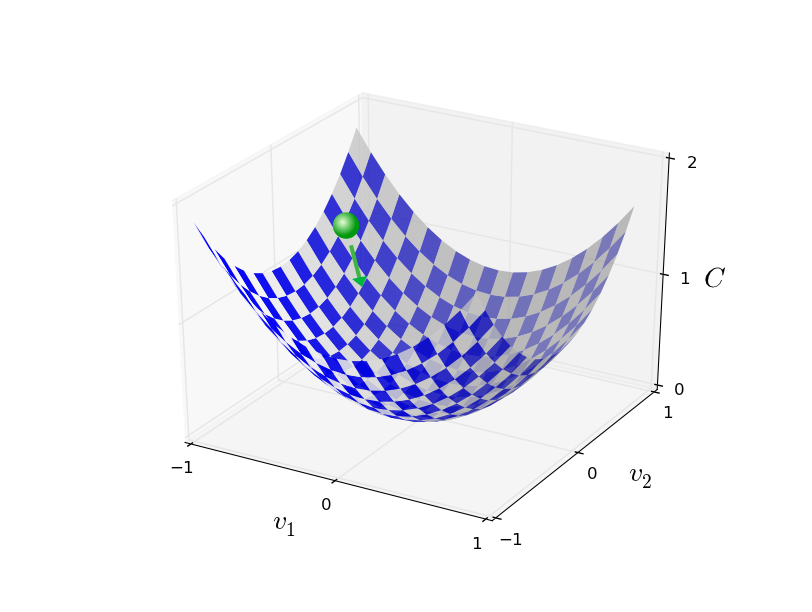
\includegraphics[width=0.903\textwidth]{images/valley_with_ball.png}
\end{center}

\noindent 注意，使用这个规则，梯度下降并不再现真实的物理运动. 在现实生活中，小球具有动量\label{term:35}，这种动量可能使它滚过斜坡，甚至（暂时地）滚上坡. 只有在摩擦效应起作用之后，小球才保证滚入山谷. 相比之下，我们选择 $\Delta v$ 的规则只是说``现在就往下走''. 对于寻找最小值来说，这仍然是一个相当不错的规则！

为了使梯度下降正确工作，我们需要选择学习率\label{term:36} $\eta$ 足够小，使得方程 (9)

\begin{align*}
\Delta C \approx \nabla C \cdot \Delta v \nonumber
\end{align*}

\noindent 是一个好的近似. 如果不这样做，我们可能最终得到 $\Delta C > 0$，这显然不好！同时，我们也不希望 $\eta$ 太小，因为那会使变化量 $\Delta v$ 非常微小，从而使梯度下降算法工作得非常缓慢. 在实际实现中，$\eta$ 经常被调整，以使方程 (9)

\begin{align*}
\Delta C \approx \nabla C \cdot \Delta v \nonumber
\end{align*}

\noindent 保持为一个好的近似，但算法又不会太慢. 我们稍后会看到这是如何工作的.

我已经解释了当 $C$ 只是两个变量的函数时的梯度下降. 但实际上，即使 $C$ 是更多变量的函数，一切也同样适用. 特别地，假设 $C$ 是 $m$ 个变量 $v_1,\ldots,v_m$ 的函数. 那么由微小变化 $\Delta v = (\Delta v_1, \ldots, \Delta v_m)^T$ 产生的 $C$ 的变化 $\Delta C$ 为

\begin{equation}
\Delta C \approx \nabla C \cdot \Delta v,
\tag{12}
\end{equation}

\noindent 其中梯度 $\nabla C$ 是向量

\begin{equation}
\nabla C \equiv \left(\frac{\partial C}{\partial v_1}, \ldots, \frac{\partial C}{\partial v_m}\right)^T.
\tag{13}
\end{equation}

\noindent 正如两变量的情况一样，我们可以选择

\begin{equation}
\Delta v = -\eta \nabla C,
\tag{14}
\end{equation}

\noindent 并且我们保证我们的（近似）表达式 (12)

\begin{align*}
\Delta C \approx \nabla C \cdot \Delta v \nonumber
\end{align*}

\noindent 对于 $\Delta C$ 将是负的. 这给了我们一种沿着梯度到达最小值的方法，即使 $C$ 是许多变量的函数，通过反复应用更新规则

\begin{equation}
v \rightarrow v' = v-\eta \nabla C.
\tag{15}
\end{equation}

\noindent 你可以把这个更新规则看作是在\emph{定义}梯度下降算法. 它给了我们一种反复改变位置 $v$ 以找到函数 $C$ 的最小值的方法. 这个规则并不总是有效——有几件事可能出错并阻止梯度下降找到 $C$ 的全局最小值，这一点我们将在后面的章节中回来探讨. 但在实践中，梯度下降通常工作得非常好，在神经网络中我们会发现它是最小化代价函数、从而帮助网络学习的一种强大方法.

事实上，从某种意义上说，梯度下降甚至是搜索最小值的\emph{最优}策略. 让我们假设我们试图在位置上移动 $\Delta v$ 以尽可能多地减小 $C$. 这等价于最小化 $\Delta C \approx \nabla C \cdot \Delta v$. 我们将移动的大小约束为 $\| \Delta v \| = \epsilon$，其中 $\epsilon > 0$ 是某个小的固定值. 换句话说，我们想要一个固定大小的小步移动，并且我们试图找到使 $C$ 减小最多的移动方向. 可以证明，使 $\nabla C \cdot \Delta v$ 最小化的 $\Delta v$ 的选择是 $\Delta v = - \eta \nabla C$，其中 $\eta = \epsilon / \|\nabla C\|$ 由大小约束 $\|\Delta v\| = \epsilon$ 确定. 因此，梯度下降可以看作是在最能使 $C$ 立即减小的方向上迈出小步的一种方式.

\begin{exerciseBox}{练习}

\begin{itemize}

\item 证明上一段的论断. \emph{提示：}如果你还不熟悉 Cauchy-Schwarz 不等式，熟悉它可能会有所帮助.

\item 我解释了当 $C$ 是两个变量的函数时以及当它是多于两个变量的函数时的梯度下降. 当 $C$ 只是一个变量的函数时会发生什么？你能给出一维情况下梯度下降在做什么的几何解释吗？

\end{itemize}

人们已经研究了许多梯度下降的变体，包括更接近模拟真实物理小球的变体. 这些模拟小球的变体有一些优点，但也有一个主要缺点：事实证明，必须计算 $C$ 的二阶偏导数，而这可能相当昂贵. 要理解为什么昂贵，假设我们想计算所有的二阶偏导数 $\partial^2 C/ \partial v_j \partial v_k$. 如果有一百万个这样的 $v_j$ 变量，那么我们需要计算大约一万亿（即一百万的平方）个二阶偏导数*\footnote{实际上，更像是半万亿，因为 $\partial^2 C/ \partial v_j \partial v_k = \partial^2 C/ \partial v_k \partial v_j$. 不过，你明白意思了.}！这在计算上将是昂贵的. 话虽如此，有一些技巧可以避免这类问题，寻找梯度下降的替代方法也是一个活跃的研究领域. 但在本书中，我们将使用梯度下降（及其变体）作为我们在神经网络中学习的主要方法.

我们如何应用梯度下降来在神经网络中学习？思路是使用梯度下降来找到使方程 (6) 中的代价最小化的权重 $w_k$ 和偏置 $b_l$

\begin{align*}
C(w,b) \equiv \frac{1}{2n} \sum_x \| y(x) - a\|^2 \nonumber
\end{align*}

\noindent. 要了解这是如何工作的，让我们重新表述梯度下降更新规则，用权重和偏置替换变量 $v_j$. 换句话说，我们的``位置''现在有分量 $w_k$ 和 $b_l$，梯度向量 $\nabla C$ 有相应的分量 $\partial C / \partial w_k$ 和 $\partial C / \partial b_l$. 按分量写出梯度下降更新规则，我们有

\begin{align}
w_k &\rightarrow w_k' = w_k-\eta \frac{\partial C}{\partial w_k} \tag{16} \\ b_l &\rightarrow b_l' = b_l-\eta \frac{\partial C}{\partial b_l}. \tag{17}
\end{align}

\noindent 通过反复应用这个更新规则，我们可以``滚下山坡''，并有望找到代价函数的最小值. 换句话说，这是一个可用于在神经网络中学习的规则.

应用梯度下降规则存在许多挑战. 我们将在后面的章节中深入探讨这些. 但現在我只想提一个问题. 要理解问题是什么，让我们回顾方程 (6) 中的二次代价

\begin{align*}
C(w,b) \equiv \frac{1}{2n} \sum_x \| y(x) - a\|^2 \nonumber
\end{align*}

\noindent. 注意这个代价函数的形式是 $C = \frac{1}{n} \sum_x C_x$，也就是说，它是对各个训练样本的代价 $C_x \equiv \frac{\|y(x)-a\|^2}{2}$ 的平均. 在实践中，为了计算梯度 $\nabla C$，我们需要对每个训练输入 $x$ 分别计算梯度 $\nabla C_x$，然后对它们求平均，$\nabla C = \frac{1}{n} \sum_x \nabla C_x$. 不幸的是，当训练输入的数量非常大时，这可能需要很长时间，因此学习发生得很慢.

一种叫做\emph{随机梯度下降}的想法可以用来加速学习. 这个想法是通过对随机选择的一小部分训练输入计算 $\nabla C_x$ 来估计梯度 $\nabla C$. 通过对这个小样本求平均，我们可以快速得到真实梯度 $\nabla C$ 的一个好的估计，这有助于加速梯度下降，从而加速学习.

为了使这些想法更精确，随机梯度下降的工作方式是随机抽取一小部分数量为 $m$ 的随机选择的训练输入. 我们将这些随机训练输入标记为 $X_1, X_2, \ldots, X_m$，并将它们称为一个\emph{小批量}. 只要样本大小 $m$ 足够大，我们期望 $\nabla C_{X_j}$ 的平均值将大致等于所有 $\nabla C_x$ 的平均值，即

\begin{equation}
\frac{\sum_{j=1}^m \nabla C_{X_{j}}}{m} \approx \frac{\sum_x \nabla C_x}{n} = \nabla C,
\tag{18}
\end{equation}

\noindent 其中第二个求和是对整个训练数据集进行的. 交换两边我们得到

\begin{equation}
\nabla C \approx \frac{1}{m} \sum_{j=1}^m \nabla C_{X_{j}},
\tag{19}
\end{equation}

\noindent 这证实了我们可以通过仅对随机选择的小批量\label{term:37}计算梯度来估计整体梯度.

为了将此明确地与神经网络中的学习联系起来，假设 $w_k$ 和 $b_l$ 表示我们神经网络中的权重和偏置. 那么随机梯度下降的工作方式是抽取一个随机选择的训练输入小批量，并用它们进行训练，

\begin{align}
w_k &\rightarrow w_k' = w_k-\frac{\eta}{m} \sum_j \frac{\partial C_{X_j}}{\partial w_k} \tag{20} \\ b_l &\rightarrow b_l' = b_l-\frac{\eta}{m} \sum_j \frac{\partial C_{X_j}}{\partial b_l}, \tag{21}
\end{align}

\noindent 其中求和是对当前小批量中的所有训练样本 $X_j$ 进行的. 然后我们抽取另一个随机选择的小批量并用它们进行训练. 如此继续，直到我们用完训练输入，这被称为完成一个训练\emph{轮次}. 到那时，我们用一个新训练轮次重新开始.

顺便提一下，值得注意的是，关于代价函数以及权重和偏置的小批量更新的缩放约定各不相同. 在方程 (6) 中

\begin{align*}
C(w,b) \equiv \frac{1}{2n} \sum_x \| y(x) - a\|^2 \nonumber
\end{align*}

\noindent 我们用因子 $\frac{1}{n}$ 缩放了整体代价函数. 人们有时会省略 $\frac{1}{n}$，对各个训练样本的代价求和而不是求平均. 当训练样本的总数事先未知时，这特别有用. 例如，如果更多的训练数据正在实时生成，就可能出现这种情况. 类似地，小批量更新规则 (20)

\begin{align*}
w_k &\rightarrow w_k' = w_k-\frac{\eta}{m} \sum_j \frac{\partial C_{X_j}}{\partial w_k} \nonumber
\end{align*}

\noindent 和 (21)

\begin{align*}
b_l &\rightarrow b_l' = b_l-\frac{\eta}{m} \sum_j \frac{\partial C_{X_j}}{\partial b_l} \nonumber
\end{align*}

\noindent 有时会省略求和前面的 $\frac{1}{m}$ 项. 从概念上讲，这几乎没有区别，因为它等价于重新缩放学习率 $\eta$. 但在对不同工作进行详细比较时，值得注意这一点.

我们可以把随机梯度下降想象成类似于政治民意调查：对一个小批量进行采样比将梯度下降应用于整个批次要容易得多，就像进行一项民意调查比进行一场完整选举要容易一样. 例如，如果我们有一个大小为 $n = 60,000$ 的训练集，就像在 MNIST 中那样，并选择（比如说）$m = 10$ 的小批量大小，这意味着我们在估计梯度时将获得 $6,000$ 倍的加速！当然，这个估计不会是完美的——会有统计波动——但它不需要完美：我们真正关心的是朝着有助于减小 $C$ 的大致方向移动，这意味着我们不需要精确计算梯度. 在实践中，随机梯度下降是神经网络学习中一种常用且强大的技术，它是我们将在本书中开发的 most 学习技术的基础.

\end{exerciseBox}
\begin{exerciseBox}{练习}

\begin{itemize}

\item 梯度下降的一个极端版本是只使用大小为 1 的小批量. 也就是说，给定一个训练输入 $x$，我们根据规则 $w_k \rightarrow w_k' = w_k - \eta \partial C_x / \partial w_k$ 和 $b_l \rightarrow b_l' = b_l - \eta \partial C_x / \partial b_l$ 来更新权重和偏置. 然后我们选择另一个训练输入，再次更新权重和偏置. 如此反复进行. 这个过程被称为\emph{在线}学习、\emph{联机}学习或\emph{增量}学习. 在在线学习中，神经网络每次只从一个训练输入中学习（就像人类一样）. 与使用小批量大小比如 $20$ 的随机梯度下降相比，请说出在线学习的一个优点和一个缺点.

\end{itemize}

让我通过讨论一个有时会困扰梯度下降初学者的观点来结束本节. 在神经网络中，代价 $C$ 当然是许多变量——所有权重和偏置——的函数，因此在某种意义上定义了一个非常高维空间中的曲面. 有些人会纠结于这样的想法：``嘿，我必须能够可视化所有这些额外的维度''. 他们可能会开始担心：``我无法在四维中思考，更不用说五维（或五百万维）了''. 他们是否缺少某种特殊能力，某种``真正的''超级数学家才有的能力？当然，答案是否定的. 即使是大多数专业数学家也无法很好地可视化四维，甚至完全不能. 他们使用的技巧是发展其他方式来表示正在发生的事情. 这正是我们上面所做的：我们使用 $\Delta C$ 的代数（而非视觉）表示来弄清楚如何移动以减少 $C$. 擅长在高维中思考的人拥有一个包含许多不同技巧的心智库；我们的代数技巧只是其中一个例子. 这些技巧可能不像我们习惯的三维可视化那样简单，但一旦你建立了这样的技巧库，你就能相当擅长在高维中思考. 我在这里不会深入更多细节，但如果你感兴趣，你可能会喜欢阅读这个关于专业数学家用于在高维中思考的一些技巧的讨论. 虽然讨论的一些技巧相当复杂，但许多最好的内容是直观且易于理解的，任何人都可以掌握.

\end{exerciseBox}
\sectionTitle{实现识别数字的网络}{实现识别数字的网络}

好的，让我们编写一个程序，使用随机梯度下降和 MNIST 训练数据来学习如何识别手写数字. 我们将用一个简短的 Python（2.7）程序来完成这件事，只有 74 行代码！我们首先需要获取 MNIST 数据. 如果你是 \texttt{git} 用户，那么你可以通过克隆本书的代码仓库来获得数据，

\begin{lstlisting}
git clone https://github.com/mnielsen/neural-networks-and-deep-learning.git

\end{lstlisting}

如果你不使用 \texttt{git}，那么你可以在这里下载数据和代码.

顺便提一下，我之前描述 MNIST 数据时，说它被分为 60,000 张训练图像和 10,000 张测试图像. 那是 MNIST 的官方描述. 实际上，我们将以稍微不同的方式划分数据. 我们会保持测试图像不变，但将 60,000 张图像的 MNIST 训练集分成两部分：一个包含 50,000 张图像的集合，我们将用它来训练我们的神经网络，以及一个单独的 10,000 张图像的\emph{验证集}. 本章中我们不会使用验证数据\label{term:38}，但在本书后面我们会发现它有助于弄清楚如何设置神经网络的某些\emph{超参数}——比如学习率等等，这些参数不是由我们的学习算法直接选择的. 尽管验证数据不是原始 MNIST 规范的一部分，但许多人以这种方式使用 MNIST，而且验证数据的使用在神经网络中很常见. 从现在起，当我提到``MNIST 训练数据''时，我指的是我们的 50,000 张图像数据集，而不是原始的 60,000 张图像数据集*\footnote{如前所述，MNIST 数据集基于 NIST（美国国家标准与技术研究院）收集的两个数据集. 为了构建 MNIST，Yann LeCun、Corinna Cortes 和 Christopher J. C. Burges 对 NIST 数据集进行了精简，并将其转换为更方便的格式. 更多细节请参见此链接. 我的仓库中的数据以一种便于在 Python 中加载和操作 MNIST 数据的形式存在. 我从蒙特利尔大学的 LISA 机器学习实验室（链接）获得了这种特定形式的数据.}.

除了 MNIST 数据之外，我们还需要一个名为 Numpy 的 Python 库，用于进行快速线性代数运算. 如果你还没有安装 Numpy，可以在这里获取.

在下面给出完整代码清单之前，让我先解释神经网络代码的核心特性. 核心是一个 \texttt{Network} 类，我们用它来表示一个神经网络. 下面是我们用来初始化一个 \texttt{Network} 对象的代码：

\begin{lstlisting}
class Network(object):

    def __init__(self, sizes):
        self.num_layers = len(sizes)
        self.sizes = sizes
        self.biases = [np.random.randn(y, 1) for y in sizes[1:]]
        self.weights = [np.random.randn(y, x)
                        for x, y in zip(sizes[:-1], sizes[1:])]

\end{lstlisting}

在这段代码中，列表 \texttt{sizes} 包含各层中神经元的数量. 例如，如果我们想创建一个 \texttt{Network} 对象，第一层有 2 个神经元，第二层有 3 个神经元，最后一层有 1 个神经元，我们可以用以下代码来实现：

\begin{lstlisting}
net = Network([2, 3, 1])

\end{lstlisting}

Network 对象中的偏置和权重都是随机初始化\label{term:39}的，使用 Numpy 的 np.random.randn 函数生成均值为 $0$、标准差\label{term:40}为 $1$ 的高斯分布. 这种随机初始化为我们的随机梯度下降算法提供了一个起点. 在后面的章节中，我们会找到更好的权重和偏置初始化方法，但目前这样就可以了. 注意，Network 的初始化代码假设第一层神经元是输入层，并省略了为这些神经元设置任何偏置，因为偏置只用于计算后续层的输出.

还要注意，偏置和权重存储为 Numpy 矩阵的列表. 例如，\texttt{net.weights[1]} 是一个 Numpy 矩阵，存储连接第二层和第三层神经元的权重. （它不是第一层和第二层，因为 Python 的列表索引从 \texttt{0} 开始.）由于 \texttt{net.weights[1]} 写起来比较冗长，我们就用 $w$ 来表示这个矩阵\label{term:41}. 它是一个矩阵，其中 $w_{jk}$ 是第二层第 $k$ 个神经元与第三层第 $j$ 个神经元之间连接的权重. 这种 $j$ 和 $k$ 索引的顺序可能看起来有些奇怪——把 $j$ 和 $k$ 索引互换一下不是更合理吗？使用这种顺序的最大好处是，它意味着第三层神经元的激活值向量为：

\begin{equation}
a' = \sigma(w a + b).
\tag{22}
\end{equation}

\noindent 这个方程中包含了不少内容，让我们逐块拆解. $a$ 是第二层神经元的激活值向量. 为了得到 $a'$，我们将 $a$ 乘以权重矩阵 $w$，再加上偏置向量 $b$. 然后我们对向量 $w a + b$ 中的每个元素逐元素地应用函数 $\sigma$. （这被称为函数 $\sigma$ 的\emph{向量化}.）很容易验证，方程 (22)

\begin{align*}
a' = \sigma(w a + b) \nonumber
\end{align*}

\noindent 与我们之前计算 S 型神经元输出的规则，即方程 (4)

\begin{align*}
\frac{1}{1+\exp(-\sum_j w_j x_j-b)} \nonumber
\end{align*}

\noindent 给出相同的结果.

\begin{exerciseBox}{练习}

\begin{itemize}

\item
将方程 (22)

\begin{align*}
a' = \sigma(w a + b) \nonumber
\end{align*}

写成分量形式，并验证它与计算 S 型神经元输出的规则 (4)

\begin{align*}
\frac{1}{1+\exp(-\sum_j w_j x_j-b)} \nonumber
\end{align*}

给出相同的结果.

\end{itemize}

有了这些认识，编写计算 \texttt{Network} 实例输出的代码就很容易了. 我们首先定义 S 型函数：

\begin{lstlisting}
def sigmoid(z):
    return 1.0/(1.0+np.exp(-z))

\end{lstlisting}

注意，当输入 z 是向量或 Numpy 数组时，Numpy 会自动逐元素地应用 sigmoid 函数，即以向量化形式应用.

然后我们给 \texttt{Network} 类添加一个 \texttt{feedforward} 方法，给定网络的输入 \texttt{a}，它返回相应的输出*\footnote{这里假设输入 \texttt{a} 是一个 \texttt{(n, 1)} 的 Numpy ndarray，而不是 \texttt{(n,)} 向量. 这里，\texttt{n} 是网络的输入数量. 如果你尝试使用 \texttt{(n,)} 向量作为输入，你会得到奇怪的结果. 尽管使用 \texttt{(n,)} 向量看起来是更自然的选择，但使用 \texttt{(n, 1)} ndarray 使得修改代码以一次性前馈多个输入变得特别容易，这有时很方便.}. 该方法所做的就是对每一层应用方程 (22)

\begin{align*}
a' = \sigma(w a + b) \nonumber
\end{align*}

\noindent：

\begin{lstlisting}
    def feedforward(self, a):
        """Return the output of the network if "a" is input."""
        for b, w in zip(self.biases, self.weights):
            a = sigmoid(np.dot(w, a)+b)
        return a

\end{lstlisting}

当然，我们希望 \texttt{Network} 对象做的主要事情是学习. 为此，我们将给它们一个 \texttt{SGD} 方法，实现随机梯度下降. 下面是代码. 有几处地方可能看起来有些神秘，但我会在代码清单之后详细解释.

\begin{lstlisting}
    def SGD(self, training_data, epochs, mini_batch_size, eta,
            test_data=None):
        """Train the neural network using mini-batch stochastic
        gradient descent.  The "training_data" is a list of tuples
        "(x, y)" representing the training inputs and the desired
        outputs.  The other non-optional parameters are
        self-explanatory.  If "test_data" is provided then the
        network will be evaluated against the test data after each
        epoch, and partial progress printed out.  This is useful for
        tracking progress, but slows things down substantially."""
        if test_data: n_test = len(test_data)
        n = len(training_data)
        for j in xrange(epochs):
            random.shuffle(training_data)
            mini_batches = [
                training_data[k:k+mini_batch_size]
                for k in xrange(0, n, mini_batch_size)]
            for mini_batch in mini_batches:
                self.update_mini_batch(mini_batch, eta)
            if test_data:
                print "Epoch {0}: {1} / {2}".format(
                    j, self.evaluate(test_data), n_test)
            else:
                print "Epoch {0} complete".format(j)

\end{lstlisting}

\texttt{training\_\allowbreak{}data} 是一个元组列表 \texttt{(x, y)}，表示训练输入和对应的期望输出. 变量 \texttt{epochs} 和 \texttt{mini\_\allowbreak{}batch\_\allowbreak{}size} 正如你所期望的——训练的轮次数，以及采样时使用的小批量的大小. \texttt{eta} 是学习率，$\eta$. 如果提供了可选参数 \texttt{test\_\allowbreak{}data}，那么程序将在每轮训练后评估网络，并打印出部分进度. 这对于跟踪进度很有用，但会大大减慢速度.

代码的工作方式如下. 在每一轮中，它首先随机打乱训练数据，然后将其分成适当大小的小批量. 这是一种从训练数据中随机采样的简便方法. 然后对于每个 \texttt{mini\_\allowbreak{}batch}，我们应用一步梯度下降. 这是通过代码 \texttt{self.update\_\allowbreak{}mini\_\allowbreak{}batch(mini\_\allowbreak{}batch, eta)} 完成的，它根据一次梯度下降迭代来更新网络权重和偏置，仅使用 \texttt{mini\_\allowbreak{}batch} 中的训练数据. 下面是 \texttt{update\_\allowbreak{}mini\_\allowbreak{}batch} 方法的代码：

\begin{lstlisting}
    def update_mini_batch(self, mini_batch, eta):
        """Update the network's weights and biases by applying
        gradient descent using backpropagation to a single mini batch.
        The "mini_batch" is a list of tuples "(x, y)", and "eta"
        is the learning rate."""
        nabla_b = [np.zeros(b.shape) for b in self.biases]
        nabla_w = [np.zeros(w.shape) for w in self.weights]
        for x, y in mini_batch:
            delta_nabla_b, delta_nabla_w = self.backprop(x, y)
            nabla_b = [nb+dnb for nb, dnb in zip(nabla_b, delta_nabla_b)]
            nabla_w = [nw+dnw for nw, dnw in zip(nabla_w, delta_nabla_w)]
        self.weights = [w-(eta/len(mini_batch))*nw
                        for w, nw in zip(self.weights, nabla_w)]
        self.biases = [b-(eta/len(mini_batch))*nb
                       for b, nb in zip(self.biases, nabla_b)]

\end{lstlisting}

大部分工作由这一行完成

\begin{lstlisting}
            delta_nabla_b, delta_nabla_w = self.backprop(x, y)

\end{lstlisting}

这调用了所谓的反向传播\label{term:42}算法，它是一种计算代价函数梯度的快速方法. 所以 update\_\allowbreak{}mini\_\allowbreak{}batch 的工作就是为 mini\_\allowbreak{}batch 中的每个训练样本计算这些梯度，然后相应地更新 self.weights 和 self.biases.

我现在不打算展示 \texttt{self.backprop} 的代码. 我们将在下一章研究反向传播的工作原理，包括 \texttt{self.backprop} 的代码. 现在，只需假设它按所声称的方式运行，为训练样本 \texttt{x} 相关的代价返回适当的梯度.

让我们看看完整的程序，包括我上面省略的文档字符串. 除了 \texttt{self.backprop} 之外，程序是不言自明的——所有繁重的工作都在 \texttt{self.SGD} 和 \texttt{self.update\_\allowbreak{}mini\_\allowbreak{}batch} 中完成，我们已经讨论过了. \texttt{self.backprop} 方法使用了一些额外的函数来帮助计算梯度，即 \texttt{sigmoid\_\allowbreak{}prime}，它计算 $\sigma$ 函数的导数，以及 \texttt{self.cost\_\allowbreak{}derivative}，我在这里不描述. 你可以通过查看代码和文档字符串来了解这些函数的大意（也许还有细节）. 我们将在下一章详细研究它们. 注意，虽然程序看起来很长，但大部分代码是旨在使代码易于理解的文档字符串. 事实上，该程序只包含 74 行非空白、非注释代码. 所有代码都可以在 GitHub 这里找到.

\begin{lstlisting}
"""
network.py
~~~~~~~~~~

A module to implement the stochastic gradient descent learning
algorithm for a feedforward neural network.  Gradients are calculated
using backpropagation.  Note that I have focused on making the code
simple, easily readable, and easily modifiable.  It is not optimized,
and omits many desirable features.
"""

#### Libraries
# Standard library
import random

# Third-party libraries
import numpy as np

class Network(object):

    def __init__(self, sizes):
        """The list ``sizes`` contains the number of neurons in the
        respective layers of the network.  For example, if the list
        was [2, 3, 1] then it would be a three-layer network, with the
        first layer containing 2 neurons, the second layer 3 neurons,
        and the third layer 1 neuron.  The biases and weights for the
        network are initialized randomly, using a Gaussian
        distribution with mean 0, and variance 1.  Note that the first
        layer is assumed to be an input layer, and by convention we
        won't set any biases for those neurons, since biases are only
        ever used in computing the outputs from later layers."""
        self.num_layers = len(sizes)
        self.sizes = sizes
        self.biases = [np.random.randn(y, 1) for y in sizes[1:]]
        self.weights = [np.random.randn(y, x)
                        for x, y in zip(sizes[:-1], sizes[1:])]

    def feedforward(self, a):
        """Return the output of the network if ``a`` is input."""
        for b, w in zip(self.biases, self.weights):
            a = sigmoid(np.dot(w, a)+b)
        return a

    def SGD(self, training_data, epochs, mini_batch_size, eta,
            test_data=None):
        """Train the neural network using mini-batch stochastic
        gradient descent.  The ``training_data`` is a list of tuples
        ``(x, y)`` representing the training inputs and the desired
        outputs.  The other non-optional parameters are
        self-explanatory.  If ``test_data`` is provided then the
        network will be evaluated against the test data after each
        epoch, and partial progress printed out.  This is useful for
        tracking progress, but slows things down substantially."""
        if test_data: n_test = len(test_data)
        n = len(training_data)
        for j in xrange(epochs):
            random.shuffle(training_data)
            mini_batches = [
                training_data[k:k+mini_batch_size]
                for k in xrange(0, n, mini_batch_size)]
            for mini_batch in mini_batches:
                self.update_mini_batch(mini_batch, eta)
            if test_data:
                print "Epoch {0}: {1} / {2}".format(
                    j, self.evaluate(test_data), n_test)
            else:
                print "Epoch {0} complete".format(j)

    def update_mini_batch(self, mini_batch, eta):
        """Update the network's weights and biases by applying
        gradient descent using backpropagation to a single mini batch.
        The ``mini_batch`` is a list of tuples ``(x, y)``, and ``eta``
        is the learning rate."""
        nabla_b = [np.zeros(b.shape) for b in self.biases]
        nabla_w = [np.zeros(w.shape) for w in self.weights]
        for x, y in mini_batch:
            delta_nabla_b, delta_nabla_w = self.backprop(x, y)
            nabla_b = [nb+dnb for nb, dnb in zip(nabla_b, delta_nabla_b)]
            nabla_w = [nw+dnw for nw, dnw in zip(nabla_w, delta_nabla_w)]
        self.weights = [w-(eta/len(mini_batch))*nw
                        for w, nw in zip(self.weights, nabla_w)]
        self.biases = [b-(eta/len(mini_batch))*nb
                       for b, nb in zip(self.biases, nabla_b)]

    def backprop(self, x, y):
        """Return a tuple ``(nabla_b, nabla_w)`` representing the
        gradient for the cost function C_x.  ``nabla_b`` and
        ``nabla_w`` are layer-by-layer lists of numpy arrays, similar
        to ``self.biases`` and ``self.weights``."""
        nabla_b = [np.zeros(b.shape) for b in self.biases]
        nabla_w = [np.zeros(w.shape) for w in self.weights]
        # feedforward
        activation = x
        activations = [x] # list to store all the activations, layer by layer
        zs = [] # list to store all the z vectors, layer by layer
        for b, w in zip(self.biases, self.weights):
            z = np.dot(w, activation)+b
            zs.append(z)
            activation = sigmoid(z)
            activations.append(activation)
        # backward pass
        delta = self.cost_derivative(activations[-1], y) * \
            sigmoid_prime(zs[-1])
        nabla_b[-1] = delta
        nabla_w[-1] = np.dot(delta, activations[-2].transpose())
        # Note that the variable l in the loop below is used a little
        # differently to the notation in Chapter 2 of the book.  Here,
        # l = 1 means the last layer of neurons, l = 2 is the
        # second-last layer, and so on.  It's a renumbering of the
        # scheme in the book, used here to take advantage of the fact
        # that Python can use negative indices in lists.
        for l in xrange(2, self.num_layers):
            z = zs[-l]
            sp = sigmoid_prime(z)
            delta = np.dot(self.weights[-l+1].transpose(), delta) * sp
            nabla_b[-l] = delta
            nabla_w[-l] = np.dot(delta, activations[-l-1].transpose())
        return (nabla_b, nabla_w)

    def evaluate(self, test_data):
        """Return the number of test inputs for which the neural
        network outputs the correct result. Note that the neural
        network's output is assumed to be the index of whichever
        neuron in the final layer has the highest activation."""
        test_results = [(np.argmax(self.feedforward(x)), y)
                        for (x, y) in test_data]
        return sum(int(x == y) for (x, y) in test_results)

    def cost_derivative(self, output_activations, y):
        """Return the vector of partial derivatives \partial C_x /
        \partial a for the output activations."""
        return (output_activations-y)

#### Miscellaneous functions
def sigmoid(z):
    """The sigmoid function."""
    return 1.0/(1.0+np.exp(-z))

def sigmoid_prime(z):
    """Derivative of the sigmoid function."""
    return sigmoid(z)*(1-sigmoid(z))

\end{lstlisting}

这个程序识别手写数字的效果如何？好吧，让我们从加载 MNIST 数据开始. 我将使用一个小的辅助程序 \texttt{mnist\_\allowbreak{}loader.py} 来完成这件事，稍后会描述. 我们在 Python shell 中执行以下命令，

\begin{lstlisting}
>>> import mnist_loader
>>> training_data, validation_data, test_data = \
... mnist_loader.load_data_wrapper()

\end{lstlisting}

当然，这也可以在一个单独的 Python 程序中完成，但如果你是跟着做的话，在 Python shell 中做可能是最简单的.

加载 MNIST 数据后，我们将建立一个有 $30$ 个隐藏神经元的 \texttt{Network}. 我们在导入上面列出的名为 \texttt{network} 的 Python 程序之后这样做，

\begin{lstlisting}
>>> import network
>>> net = network.Network([784, 30, 10])

\end{lstlisting}

最后，我们将使用随机梯度下降从 MNIST \texttt{training\_\allowbreak{}data} 中学习 30 轮，小批量大小为 10，学习率为 $\eta = 3.0$，

\begin{lstlisting}
>>> net.SGD(training_data, 30, 10, 3.0, test_data=test_data)

\end{lstlisting}

注意，如果你一边阅读一边运行代码，执行需要一些时间——对于一台典型的机器（截至 2015 年），可能需要几分钟才能运行完. 我建议你让程序运行起来，继续阅读，并定期检查代码的输出. 如果你赶时间，可以通过减少轮次\label{term:43}数、减少隐藏神经元数量，或者只使用部分训练数据来加速. 注意，生产级别的代码会快得多：这些 Python 脚本旨在帮助你理解神经网络的工作原理，而不是高性能代码！当然，一旦我们训练好了一个网络，它确实可以在几乎任何计算平台上非常快速地运行. 例如，一旦我们为网络学习到一组好的权重和偏置，它就可以很容易地被移植到网页浏览器中的 Javascript 中运行，或者作为移动设备上的原生应用运行. 无论如何，下面是神经网络一次训练运行的输出部分记录. 该记录显示了每轮训练后神经网络正确识别的测试图像数量. 如你所见，仅仅一轮之后，这个数字就达到了 10,000 中的 9,129，而且这个数字还在继续增长，

\begin{lstlisting}
Epoch 0: 9129 / 10000
Epoch 1: 9295 / 10000
Epoch 2: 9348 / 10000
...
Epoch 27: 9528 / 10000
Epoch 28: 9542 / 10000
Epoch 29: 9534 / 10000

\end{lstlisting}

也就是说，训练后的网络给我们提供了大约 $95$ ％的分类率——峰值时达到 $95.42$ ％（``第 28 轮''）！作为第一次尝试，这相当令人鼓舞. 然而，我应该提醒你，如果你运行代码，你的结果不一定和我完全一样，因为我们将使用（不同的）随机权重和偏置来初始化我们的网络. 为了生成本章中的结果，我取的是三次运行中最好的结果.

让我们重新运行上面的实验，将隐藏神经元数量改为 $100$. 和之前一样，如果你一边阅读一边运行代码，应该注意执行需要相当长的时间（在我的机器上，这个实验每轮训练需要几十秒），所以明智的做法是在代码执行的同时继续阅读.

\begin{lstlisting}
>>> net = network.Network([784, 100, 10])
>>> net.SGD(training_data, 30, 10, 3.0, test_data=test_data)

\end{lstlisting}

果然，这将结果提高到了 $96.59$ ％. 至少在这个例子中，使用更多的隐藏神经元帮助我们获得了更好的结果*\footnote{读者反馈表明这个实验的结果有相当大的差异，有些训练运行给出的结果要差不少. 使用第 3 章介绍的技术将大大减少我们网络在不同训练运行之间的性能差异.}.

当然，为了获得这些准确率，我必须对训练轮次数、小批量大小和学习率 $\eta$ 做出具体选择. 正如我上面提到的，这些被称为我们神经网络的超参数\label{term:44}，以便将它们与我们的学习算法学到的参数（权重和偏置）区分开来. 如果我们选择超参数不当，就会得到糟糕的结果. 例如，假设我们选择了学习率 $\eta = 0.001$，

\begin{lstlisting}
>>> net = network.Network([784, 100, 10])
>>> net.SGD(training_data, 30, 10, 0.001, test_data=test_data)

\end{lstlisting}

结果就不那么令人鼓舞了，

\begin{lstlisting}
Epoch 0: 1139 / 10000
Epoch 1: 1136 / 10000
Epoch 2: 1135 / 10000
...
Epoch 27: 2101 / 10000
Epoch 28: 2123 / 10000
Epoch 29: 2142 / 10000

\end{lstlisting}

然而，你可以看到网络的性能随着时间的推移在慢慢变好. 这表明应该增大学习率，比如增加到 $\eta = 0.01$. 如果我们这样做，会得到更好的结果，这又表明应该再次增大学习率. （如果做出改变能改善情况，就尝试做得更多！）如果我们这样做几次，最终会得到大约 $\eta = 1.0$ 的学习率（也许微调到 $3.0$），这接近我们之前的实验. 所以即使我们最初对超参数的选择很差，我们至少获得了足够的信息来帮助我们改进超参数的选择.

一般来说，调试神经网络可能很有挑战性. 当初始超参数选择产生的结果不比随机噪声好时尤其如此. 假设我们尝试之前成功的 30 个隐藏神经元网络架构，但将学习率改为 $\eta = 100.0$：

\begin{lstlisting}
>>> net = network.Network([784, 30, 10])
>>> net.SGD(training_data, 30, 10, 100.0, test_data=test_data)

\end{lstlisting}

此时我们实际上走得太远了，学习率太高了：

\begin{lstlisting}
Epoch 0: 1009 / 10000
Epoch 1: 1009 / 10000
Epoch 2: 1009 / 10000
Epoch 3: 1009 / 10000
...
Epoch 27: 982 / 10000
Epoch 28: 982 / 10000
Epoch 29: 982 / 10000

\end{lstlisting}

现在想象我们是第一次遇到这个问题. 当然，我们从之前的实验中知道正确的做法是降低学习率. 但如果我们第一次遇到这个问题，那么输出中没有什么能指导我们该怎么做. 我们可能不仅担心学习率，还担心神经网络的其他各个方面. 我们可能想知道是否以某种方式初始化了权重和偏置，使得网络难以学习？或者也许我们没有足够的训练数据来获得有意义的学习？也许我们没有运行足够的轮次？或者也许具有这种架构的神经网络不可能学会识别手写数字？也许学习率太低了？或者，也许学习率太高了？当你第一次遇到一个问题时，你并不总是确定的.

从中得出的教训是，调试神经网络并非易事，而且，就像普通编程一样，它是一门艺术. 你需要学习调试的艺术，才能从神经网络中获得好的结果. 更一般地说，我们需要发展选择好的超参数和好的架构的启发式方法. 我们将在本书中详细讨论所有这些，包括我上面是如何选择超参数的.

\end{exerciseBox}
\begin{exerciseBox}{练习}

\begin{itemize}

\item 尝试创建一个只有两层的网络——一个输入层和一个输出层，没有隐藏层——分别包含 784 和 10 个神经元. 使用随机梯度下降训练该网络. 你能达到怎样的分类准确率？

\end{itemize}

前面我略过了 MNIST 数据是如何加载的细节. 这相当直接. 为了完整起见，这里是代码. 用于存储 MNIST 数据的数据结构在文档字符串中有描述——都是些简单的东西，Numpy \texttt{ndarray} 对象的元组和列表（如果你不熟悉 \texttt{ndarray}，就把它们当作向量）：

\begin{lstlisting}
"""
mnist_loader
~~~~~~~~~~~~

A library to load the MNIST image data.  For details of the data
structures that are returned, see the doc strings for ``load_data``
and ``load_data_wrapper``.  In practice, ``load_data_wrapper`` is the
function usually called by our neural network code.
"""

#### Libraries
# Standard library
import cPickle
import gzip

# Third-party libraries
import numpy as np

def load_data():
    """Return the MNIST data as a tuple containing the training data,
    the validation data, and the test data.

    The ``training_data`` is returned as a tuple with two entries.
    The first entry contains the actual training images.  This is a
    numpy ndarray with 50,000 entries.  Each entry is, in turn, a
    numpy ndarray with 784 values, representing the 28 * 28 = 784
    pixels in a single MNIST image.

    The second entry in the ``training_data`` tuple is a numpy ndarray
    containing 50,000 entries.  Those entries are just the digit
    values (0...9) for the corresponding images contained in the first
    entry of the tuple.

    The ``validation_data`` and ``test_data`` are similar, except
    each contains only 10,000 images.

    This is a nice data format, but for use in neural networks it's
    helpful to modify the format of the ``training_data`` a little.
    That's done in the wrapper function ``load_data_wrapper()``, see
    below.
    """
    f = gzip.open('../data/mnist.pkl.gz', 'rb')
    training_data, validation_data, test_data = cPickle.load(f)
    f.close()
    return (training_data, validation_data, test_data)

def load_data_wrapper():
    """Return a tuple containing ``(training_data, validation_data,
    test_data)``. Based on ``load_data``, but the format is more
    convenient for use in our implementation of neural networks.

    In particular, ``training_data`` is a list containing 50,000
    2-tuples ``(x, y)``.  ``x`` is a 784-dimensional numpy.ndarray
    containing the input image.  ``y`` is a 10-dimensional
    numpy.ndarray representing the unit vector corresponding to the
    correct digit for ``x``.

    ``validation_data`` and ``test_data`` are lists containing 10,000
    2-tuples ``(x, y)``.  In each case, ``x`` is a 784-dimensional
    numpy.ndarry containing the input image, and ``y`` is the
    corresponding classification, i.e., the digit values (integers)
    corresponding to ``x``.

    Obviously, this means we're using slightly different formats for
    the training data and the validation / test data.  These formats
    turn out to be the most convenient for use in our neural network
    code."""
    tr_d, va_d, te_d = load_data()
    training_inputs = [np.reshape(x, (784, 1)) for x in tr_d[0]]
    training_results = [vectorized_result(y) for y in tr_d[1]]
    training_data = zip(training_inputs, training_results)
    validation_inputs = [np.reshape(x, (784, 1)) for x in va_d[0]]
    validation_data = zip(validation_inputs, va_d[1])
    test_inputs = [np.reshape(x, (784, 1)) for x in te_d[0]]
    test_data = zip(test_inputs, te_d[1])
    return (training_data, validation_data, test_data)

def vectorized_result(j):
    """Return a 10-dimensional unit vector with a 1.0 in the jth
    position and zeroes elsewhere.  This is used to convert a digit
    (0...9) into a corresponding desired output from the neural
    network."""
    e = np.zeros((10, 1))
    e[j] = 1.0
    return e

\end{lstlisting}

我上面说过我们的程序得到了相当不错的结果. 这是什么意思？跟什么比算好？有一些简单的（非神经网络的）基线测试可以用来对比，这有助于理解什么叫表现良好. 最简单的基线当然就是随机猜测数字. 那大约会有百分之十的正确率. 我们做得比那好多了！

那一个不那么平凡的基线呢？让我们尝试一个极其简单的想法：我们来看一幅图像有多\emph{暗}. 例如，一个 $2$ 的图像通常会比一个 $1$ 的图像暗不少，仅仅是因为有更多的像素被涂黑，如下面的例子所示：

\begin{center}
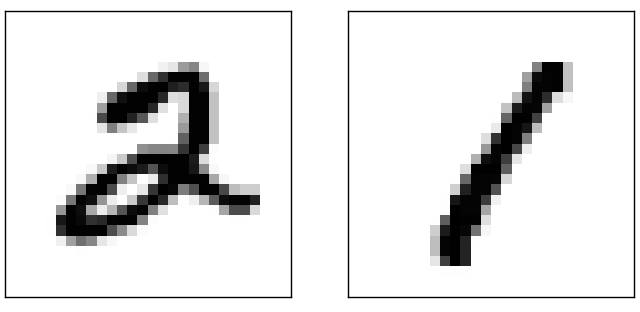
\includegraphics[width=0.427\textwidth]{images/mnist_2_and_1.png}
\end{center}

\noindent 这提示我们可以用训练数据来计算每个数字 $0, 1, 2,\ldots, 9$ 的平均暗度. 当给定一幅新图像时，我们计算该图像有多暗，然后猜测它属于平均暗度最接近的那个数字. 这是一个简单的过程，也很容易编码，所以我不会明确写出代码——如果你感兴趣，它在 GitHub 仓库中. 但它比随机猜测有了很大的改进，在 $10,000$ 幅测试图像中正确识别了 $2,225$ 幅，即 $22.25$ 的准确率.

找到其他能达到 $20$ 到 $50$ 百分比范围内准确率的想法并不困难. 如果你再努力一些，可以达到 $50$ 百分比以上. 但要获得更高的准确率，使用成熟的机器学习算法会有所帮助. 让我们尝试使用最著名的算法之一，\emph{支持向量机}或 \emph{SVM}. 如果你不熟悉 SVM，不用担心，我们不需要理解 SVM 的工作原理细节. 相反，我们将使用一个名为 scikit-learn 的 Python 库，它为被称为 LIBSVM 的快速 C 语言 SVM 库提供了一个简单的 Python 接口.

如果我们使用默认设置运行 scikit-learn 的 SVM 分类器，那么它在 10,000 幅测试图像中正确识别了 9,435 幅.（代码可在此处获得.）这比我们基于图像暗度进行分类的朴素方法有了很大的改进. 实际上，这意味着 SVM 的表现大致与我们的神经网络相当，只是稍差一点. 在后面的章节中，我们将介绍新的技术，使我们能够改进神经网络，使其表现远好于 SVM.

然而，故事并没有到此结束.10,000 幅中正确 9,435 幅的结果是 scikit-learn 对 SVM 的默认设置.SVM 有许多可调参数，并且有可能搜索出能改善这种开箱即用性能的参数. 我不会明确地进行这种搜索，而是向你推荐 Andreas Mueller 的这篇博客文章，如果你想了解更多.Mueller 表明，通过一些工作来优化 SVM 的参数，可以将性能提升到 98.5 百分比以上的准确率. 换句话说，一个调优良好的 SVM 大约每 70 个数字中只错一个. 那相当不错！神经网络能做得更好吗？

事实上，它们可以. 目前，设计良好的神经网络在解决 MNIST 问题上优于所有其他技术，包括 SVM. 当前（2013 年）的记录是正确分类 10,000 幅图像中的 9,979 幅. 这是由 Li Wan、Matthew Zeiler、Sixin Zhang、Yann LeCun 和 Rob Fergus 完成的. 我们将在本书后面看到他们使用的大部分技术. 在那个水平上，性能已经接近人类水平，甚至可以说更好，因为相当多的 MNIST 图像即使对人类来说也难以自信地识别，例如：

\begin{center}
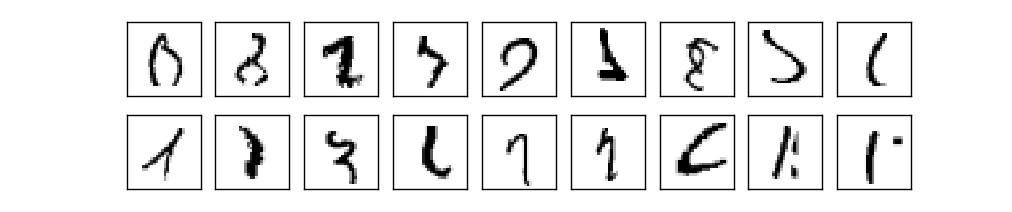
\includegraphics[width=0.933\textwidth]{images/mnist_really_bad_images.png}
\end{center}

\noindent 我相信你会同意这些图像很难分类！在 MNIST 数据集中有这样的图像的情况下，神经网络能够准确分类 10,000 幅测试图像中除 21 幅之外的所有图像，这是非常了不起的. 通常，在编程时我们认为解决像识别 MNIST 数字这样复杂的问题需要一个复杂的算法. 但即使是刚才提到的 Wan \emph{et al} 论文中的神经网络也只涉及相当简单的算法，即我们在本章中看到的算法的变体. 所有的复杂性都是从训练数据中自动学习到的. 在某种意义上，我们的结果和更复杂的论文中的结果所蕴含的寓意是，对于某些问题：复杂算法 $\leq$ 简单学习算法 + 好的训练数据.

\end{exerciseBox}
\sectionTitle{迈向深度学习}{迈向深度学习}

虽然我们的神经网络给出了令人印象深刻的表现，但这种表现多少有些神秘. 网络中的权重和偏置是自动发现的. 这意味着我们并不能立刻解释网络是如何做到它所做的事情的. 我们能否找到某种方式来理解我们的网络对手写数字进行分类所依据的原理？而且，如果有了这些原理，我们能否做得更好？

更直白地提出这些问题，假设几十年后神经网络带来了人工智能\label{term:45}（AI）. 我们会理解这些智能网络是如何工作的吗？也许这些网络对我们来说是不透明的，其中的权重和偏置我们并不理解，因为它们是自动学习出来的. 在人工智能研究的早期，人们希望构建人工智能的努力也能帮助我们理解智能背后的原理，也许还有人类大脑的运作方式. 但也许结果会是，我们最终既不理解大脑，也不理解人工智能是如何工作的！

为了回答这些问题，让我们回想一下我在本章开头给出的人工神经元的解释，即作为一种权衡证据的手段. 假设我们想确定一幅图像是否显示了一张人脸：\footnote{Credits: 1. Ester Inbar. 2. Unknown. 3. NASA, ESA, G. Illingworth, D. Magee, and P. Oesch (University of California, Santa Cruz), R. Bouwens (Leiden University), and the HUDF09 Team. Click on the images for more details.} 我们可以用处理手写数字识别的同样方式来攻克这个问题——把图像中的像素作为神经网络的输入，网络的输出是一个单独的神经元，表示``是的，这是一张脸''或``不，这不是一张脸''.

假设我们这样做，但我们不使用学习算法. 相反，我们要尝试手工设计一个网络，选择合适的权重和偏置. 我们该怎么做呢？暂时完全忘掉神经网络，我们可以使用的一个启发式方法是将问题分解为子问题：图像的左上方有眼睛吗？右上方有眼睛吗？中间有鼻子吗？下方中间有嘴巴吗？顶部有头发吗？等等.

如果其中几个问题的答案是``是''，或者甚至只是``可能是''，那么我们就会得出结论，这幅图像很可能是一张脸. 反过来，如果大多数问题的答案是``不''，那么这幅图像可能不是一张脸.

当然，这只是一个粗略的启发式方法，它有许多缺陷. 也许这个人是秃头，所以没有头发. 也许我们只能看到脸的一部分，或者脸是侧着的，所以一些面部特征被遮挡了. 尽管如此，这个启发式方法表明，如果我们能用神经网络解决这些子问题，那么也许我们可以通过组合这些子问题的网络来构建一个用于人脸检测的神经网络. 这里有一个可能的架构，矩形表示子网络. 注意，这并不是要作为解决人脸检测问题的现实方法；相反，它是为了帮助我们建立关于网络如何运作的直觉. 这是该架构：

\begin{center}
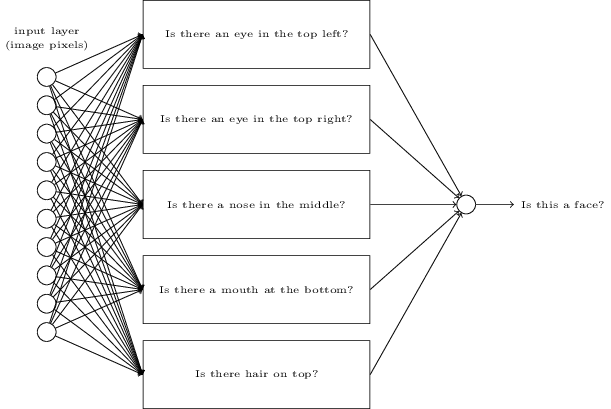
\includegraphics[width=0.9\textwidth]{images/tikz14.png}
\end{center}

\noindent 子网络也可以被分解，这也是合理的. 假设我们正在考虑这个问题：``左上方有眼睛吗？'' 这可以分解为诸如：``有眉毛吗？''；``有睫毛吗？''；``有虹膜吗？''；等等. 当然，这些问题实际上还应该包括位置信息——``眉毛在左上方，并且在虹膜上方吗？''，诸如此类——但让我们保持简单. 回答``左上方有眼睛吗？''这个问题的网络现在可以分解为：

\begin{center}
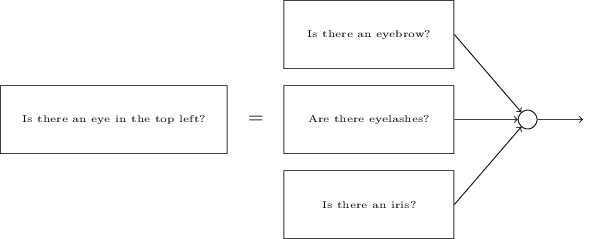
\includegraphics[width=0.9\textwidth]{images/tikz15.png}
\end{center}

\noindent 这些问题也可以被进一步分解，通过多个层越来越深入. 最终，我们将使用那些回答非常简单问题的子网络，这些问题简单到可以很容易地在单个像素的层面上回答. 例如，这些问题可能是关于图像中特定位置上是否存在非常简单的形状. 这样的问题可以由连接到图像中原始像素的单个神经元来回答.

最终结果是一个网络，它把一个非常复杂的问题——这幅图像是否显示了一张脸——分解为可以在单个像素层面上回答的非常简单的问题. 它通过一系列许多层来做到这一点，早期的层回答关于输入图像的非常简单和具体的问题，而后面的层则构建起一个越来越复杂和抽象的概念层次结构. 具有这种多层结构——两个或更多隐藏层——的网络被称为\emph{深度神经网络}.

当然，我还没有说明如何进行这种递归地分解为子网络. 手工设计网络中的权重和偏置当然是不切实际的. 相反，我们希望使用学习算法，使网络能够从训练数据中自动学习权重和偏置——从而学习概念的层次结构.20 世纪 80 年代和 90 年代的研究人员尝试使用随机梯度下降和反向传播来训练深度网络. 不幸的是，除了少数特殊架构外，他们并没有取得多大成功. 网络会学习，但非常缓慢，在实践中往往慢到没有用处.

自 2006 年以来，一系列技术被开发出来，使得在深度神经网络中进行学习成为可能. 这些深度学习技术基于随机梯度下降和反向传播，但也引入了新的思想. 这些技术使得训练更深（也更大）的网络成为可能——人们现在经常训练具有 5 到 10 个隐藏层的网络. 而且，事实证明，在许多问题上，这些网络的表现远远优于浅层神经网络，即只有一个隐藏层的网络. 原因当然是深度网络能够构建复杂的概念层次结构. 这有点像是传统编程语言使用模块化设计和抽象思想来创建复杂计算机程序的方式. 把深度网络与浅层网络进行比较，有点像是把一种能够进行函数调用的编程语言与一种被剥夺了这种调用能力的精简语言进行比较. 抽象在神经网络中采取的形式与传统编程中不同，但它同样重要.
